% ==================== UNIDAD II ====================
% Derivadas Parciales

\section{Unidad II: Derivadas Parciales}

\begin{TemaBox}[Derivadas Parciales: Concepto fundamental]
Las derivadas parciales extienden el concepto de derivada a funciones de varias variables, permitiéndonos estudiar cómo cambia una función cuando variamos una sola variable mientras mantenemos las demás constantes. Este concepto es fundamental en física, ingeniería, economía y todas las áreas donde interactúan múltiples variables.
\end{TemaBox}

\subsection{La derivada parcial}

\paragraph{Introducción.}
En cálculo de una variable, la derivada \(\frac{dy}{dx}\) mide la razón de cambio de \(y\) con respecto a \(x\). Para funciones de varias variables, necesitamos un concepto similar que nos permita medir cómo cambia la función cuando variamos una variable a la vez.

Consideremos una función \(z = f(x,y)\) de dos variables. Podemos estudiar cómo cambia \(z\) cuando:
\begin{itemize}
  \item Variamos \(x\) manteniendo \(y\) constante
  \item Variamos \(y\) manteniendo \(x\) constante
\end{itemize}

\begin{InfoBox}
\Meta{Definición}{La \textbf{derivada parcial} de \(f\) con respecto a \(x\) se denota \(\frac{\partial f}{\partial x}\) o \(f_x\), y se calcula derivando con respecto a \(x\) tratando \(y\) como constante.}

\Meta{Notación}{Para \(z = f(x,y)\) usamos:}
\begin{itemize}
  \item \(\frac{\partial f}{\partial x}\), \(\frac{\partial z}{\partial x}\), \(f_x(x,y)\), o \(z_x\)
  \item \(\frac{\partial f}{\partial y}\), \(\frac{\partial z}{\partial y}\), \(f_y(x,y)\), o \(z_y\)
\end{itemize}
\end{InfoBox}

\paragraph{Definición formal.}
Sea \(z = f(x,y)\) una función de dos variables. Las derivadas parciales se definen como:

\[
\frac{\partial f}{\partial x} = \lim_{h \to 0} \frac{f(x+h, y) - f(x,y)}{h}
\]

\[
\frac{\partial f}{\partial y} = \lim_{h \to 0} \frac{f(x, y+h) - f(x,y)}{h}
\]

\paragraph{Interpretación geométrica.}
\begin{itemize}
  \item \(\frac{\partial f}{\partial x}\) representa la pendiente de la curva formada al intersectar la superficie \(z=f(x,y)\) con un plano \(y=\text{constante}\)
  \item \(\frac{\partial f}{\partial y}\) representa la pendiente de la curva formada al intersectar la superficie \(z=f(x,y)\) con un plano \(x=\text{constante}\)
\end{itemize}

\paragraph{Ejemplos resueltos.}

\begin{EjercicioBox}[Ejemplo 1: Función polinomial]
Calcular las derivadas parciales de \(f(x,y) = x^3 + 2xy^2 - y^3\).

\textbf{Solución:}

\textbf{Para} \(\frac{\partial f}{\partial x}\): Tratamos \(y\) como constante
\begin{align*}
\frac{\partial f}{\partial x} &= \frac{\partial}{\partial x}(x^3 + 2xy^2 - y^3) \\
&= 3x^2 + 2y^2 \cdot 1 - 0 \\
&= \boxed{3x^2 + 2y^2}
\end{align*}

\textbf{Para} \(\frac{\partial f}{\partial y}\): Tratamos \(x\) como constante
\begin{align*}
\frac{\partial f}{\partial y} &= \frac{\partial}{\partial y}(x^3 + 2xy^2 - y^3) \\
&= 0 + 2x \cdot 2y - 3y^2 \\
&= \boxed{4xy - 3y^2}
\end{align*}
\end{EjercicioBox}

\begin{EjercicioBox}[Ejemplo 2: Función con exponencial]
Calcular las derivadas parciales de \(f(x,y) = e^{xy} + \sin(x) \cos(y)\).

\textbf{Solución:}

\textbf{Para} \(\frac{\partial f}{\partial x}\):
\begin{align*}
\frac{\partial f}{\partial x} &= \frac{\partial}{\partial x}(e^{xy} + \sin(x)\cos(y)) \\
&= e^{xy} \cdot y + \cos(x) \cdot \cos(y) \\
&= \boxed{ye^{xy} + \cos(x)\cos(y)}
\end{align*}

\textbf{Para} \(\frac{\partial f}{\partial y}\):
\begin{align*}
\frac{\partial f}{\partial y} &= \frac{\partial}{\partial y}(e^{xy} + \sin(x)\cos(y)) \\
&= e^{xy} \cdot x + \sin(x) \cdot (-\sin(y)) \\
&= \boxed{xe^{xy} - \sin(x)\sin(y)}
\end{align*}
\end{EjercicioBox}

\begin{EjercicioBox}[Ejemplo 3: Función racional]
Calcular las derivadas parciales de \(f(x,y) = \frac{x^2 + y^2}{x - y}\).

\textbf{Solución:}

\textbf{Para} \(\frac{\partial f}{\partial x}\): Usamos la regla del cociente
\begin{align*}
\frac{\partial f}{\partial x} &= \frac{(x-y)\frac{\partial}{\partial x}(x^2+y^2) - (x^2+y^2)\frac{\partial}{\partial x}(x-y)}{(x-y)^2} \\
&= \frac{(x-y)(2x) - (x^2+y^2)(1)}{(x-y)^2} \\
&= \frac{2x^2 - 2xy - x^2 - y^2}{(x-y)^2} \\
&= \boxed{\frac{x^2 - 2xy - y^2}{(x-y)^2}}
\end{align*}

\textbf{Para} \(\frac{\partial f}{\partial y}\):
\begin{align*}
\frac{\partial f}{\partial y} &= \frac{(x-y)\frac{\partial}{\partial y}(x^2+y^2) - (x^2+y^2)\frac{\partial}{\partial y}(x-y)}{(x-y)^2} \\
&= \frac{(x-y)(2y) - (x^2+y^2)(-1)}{(x-y)^2} \\
&= \frac{2xy - 2y^2 + x^2 + y^2}{(x-y)^2} \\
&= \boxed{\frac{x^2 + 2xy - y^2}{(x-y)^2}}
\end{align*}
\end{EjercicioBox}

\begin{EjercicioBox}[Ejemplo 4: Función de tres variables]
Calcular las derivadas parciales de \(f(x,y,z) = x^2yz + xy^2z + xyz^2\).

\textbf{Solución:}

\textbf{Para} \(\frac{\partial f}{\partial x}\):
\begin{align*}
\frac{\partial f}{\partial x} &= 2xyz + y^2z + yz^2 = \boxed{yz(2x + y + z)}
\end{align*}

\textbf{Para} \(\frac{\partial f}{\partial y}\):
\begin{align*}
\frac{\partial f}{\partial y} &= x^2z + 2xyz + xz^2 = \boxed{xz(x + 2y + z)}
\end{align*}

\textbf{Para} \(\frac{\partial f}{\partial z}\):
\begin{align*}
\frac{\partial f}{\partial z} &= x^2y + xy^2 + 2xyz = \boxed{xy(x + y + 2z)}
\end{align*}
\end{EjercicioBox}

\paragraph{Aplicaciones prácticas.}
Las derivadas parciales tienen aplicaciones en:
\begin{itemize}
  \item \textbf{Física:} Ecuaciones de calor, ondas y difusión
  \item \textbf{Economía:} Utilidad marginal, productividad marginal
  \item \textbf{Ingeniería:} Análisis de sensibilidad en diseño
  \item \textbf{Estadística:} Optimización de funciones de verosimilitud
  \item \textbf{Machine Learning:} Gradiente descendente en redes neuronales
\end{itemize}

\subsubsection{Construcción geométrica de la derivada parcial con software}

\begin{TemaBox}[Visualización geométrica de derivadas parciales]
La interpretación geométrica de las derivadas parciales nos permite comprender cómo se comporta una superficie tridimensional al realizar cortes paralelos a los planos coordenados. Cada derivada parcial representa la pendiente de una curva resultante de estas intersecciones.
\end{TemaBox}

\paragraph{Concepto geométrico fundamental.}

Para una función \(z = f(x,y)\) que representa una superficie en el espacio tridimensional:

\begin{itemize}
  \item \(\frac{\partial f}{\partial x}\) en \((x_0, y_0)\) es la pendiente de la curva de intersección entre la superficie y el plano \(y = y_0\)
  \item \(\frac{\partial f}{\partial y}\) en \((x_0, y_0)\) es la pendiente de la curva de intersección entre la superficie y el plano \(x = x_0\)
\end{itemize}

\paragraph{Visualización paso a paso.}

Consideremos la función \(f(x,y) = x^2 + y^2\) (un paraboloide). Vamos a visualizar cómo se construyen geométricamente sus derivadas parciales.

\begin{figure}[h!]
\centering
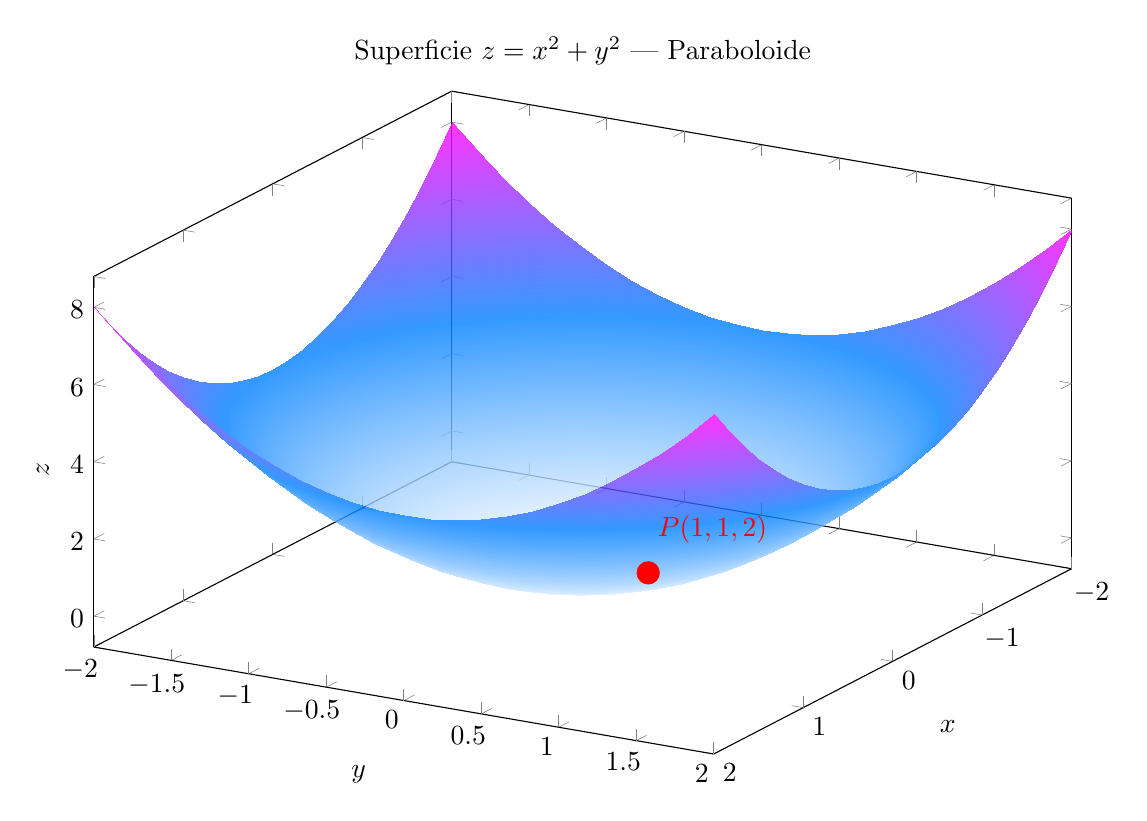
\begin{tikzpicture}
  \begin{axis}[
      view={120}{30},
      width=14cm, height=10cm,
      xlabel={$x$}, ylabel={$y$}, zlabel={$z$},
      domain=-2:2, y domain=-2:2,
      samples=25, samples y=25,
      colormap/cool,
      title={Superficie \(z = x^2 + y^2\) — Paraboloide}
  ]
    % Superficie principal
    \addplot3[surf,opacity=0.8,shader=interp] {x^2 + y^2};
    
    % Punto de interés
    \addplot3[only marks, mark=*, mark size=4pt, color=red] coordinates {(1,1,2)};
    \node[anchor=south west] at (axis cs:1,1,2.5) {\textcolor{red}{$P(1,1,2)$}};
  \end{axis}
\end{tikzpicture}
\caption{Superficie \(z = f(x,y) = x^2 + y^2\) con punto de interés \(P(1,1,2)\).}
\label{fig:superficie_base}
\end{figure}

\paragraph{Derivada parcial respecto a \(x\): Corte con \(y = \text{constante}\).}

Cuando fijamos \(y = 1\), la superficie se reduce a una curva en el plano \(y = 1\):
\[
z = f(x,1) = x^2 + 1
\]

La derivada parcial en \((1,1)\) es:
\[
\frac{\partial f}{\partial x}\bigg|_{(1,1)} = 2x\bigg|_{x=1} = 2
\]

Esto significa que la pendiente de la curva en el punto \(P\) es 2 cuando nos movemos en la dirección \(x\).

\begin{figure}[h!]
\centering
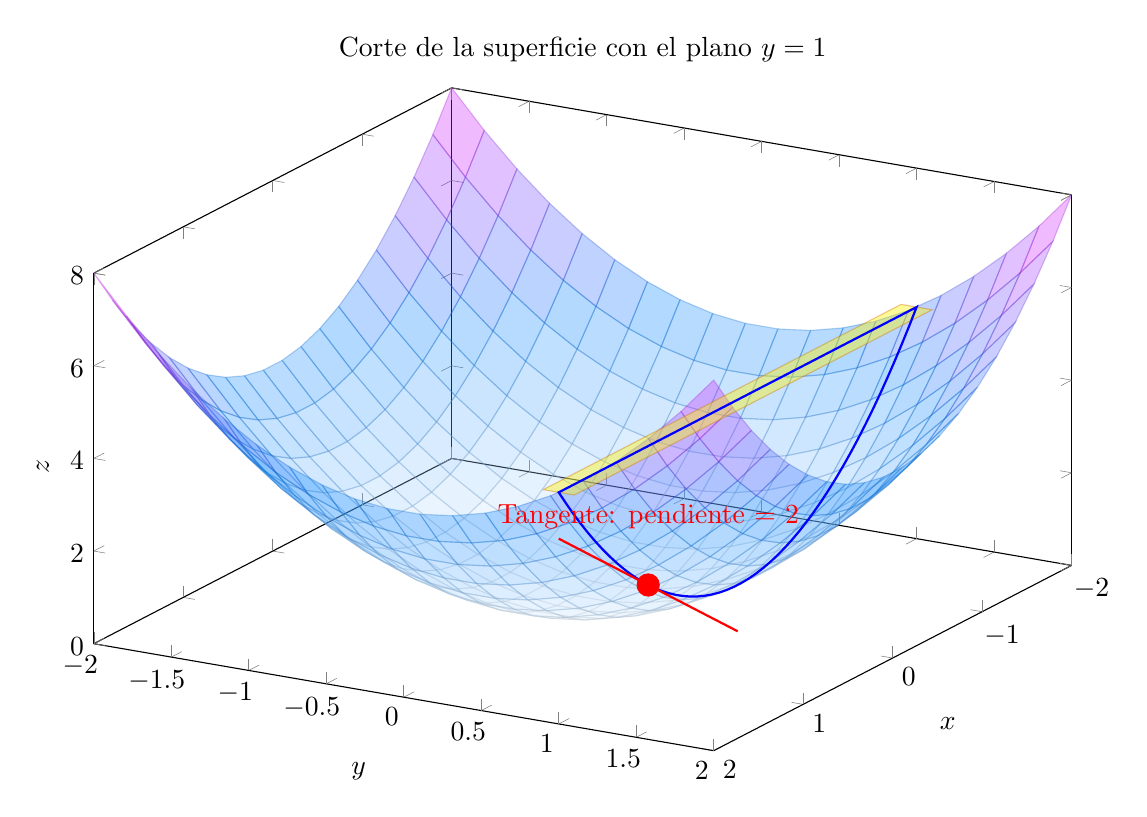
\begin{tikzpicture}
  \begin{axis}[
      view={120}{30},
      width=14cm, height=10cm,
      xlabel={$x$}, ylabel={$y$}, zlabel={$z$},
      xmin=-2, xmax=2, ymin=-2, ymax=2, zmin=0, zmax=8,
      title={Corte de la superficie con el plano \(y=1\)}
  ]
    % Superficie translúcida
    \addplot3[surf,opacity=0.3,colormap/cool,domain=-2:2, y domain=-2:2,samples=20] {x^2 + y^2};
    
    % Plano y=1
    \addplot3[surf,opacity=0.4,color=yellow,domain=-2:2,y domain=0.9:1.1,samples=2] {x^2 + 1};
    
    % Curva de intersección y=1
    \addplot3[thick,color=blue,domain=-2:2,samples=50] (x,1,{x^2 + 1});
    
    % Punto de tangencia
    \addplot3[only marks, mark=*, mark size=4pt, color=red] coordinates {(1,1,2)};
    
    % Recta tangente con pendiente 2
    \addplot3[thick,color=red,domain=0:2,samples=2] (x,1,{2*(x-1) + 2});
    
    \node[anchor=south] at (axis cs:1,1,3) {\textcolor{red}{Tangente: pendiente = 2}};
  \end{axis}
\end{tikzpicture}
\caption{Curva azul: intersección con \(y=1\). Recta roja: tangente con pendiente \(\frac{\partial f}{\partial x} = 2\).}
\label{fig:corte_x}
\end{figure}

\paragraph{Derivada parcial respecto a \(y\): Corte con \(x = \text{constante}\).}

Cuando fijamos \(x = 1\), la superficie se reduce a:
\[
z = f(1,y) = 1 + y^2
\]

La derivada parcial en \((1,1)\) es:
\[
\frac{\partial f}{\partial y}\bigg|_{(1,1)} = 2y\bigg|_{y=1} = 2
\]

\begin{figure}[h!]
\centering
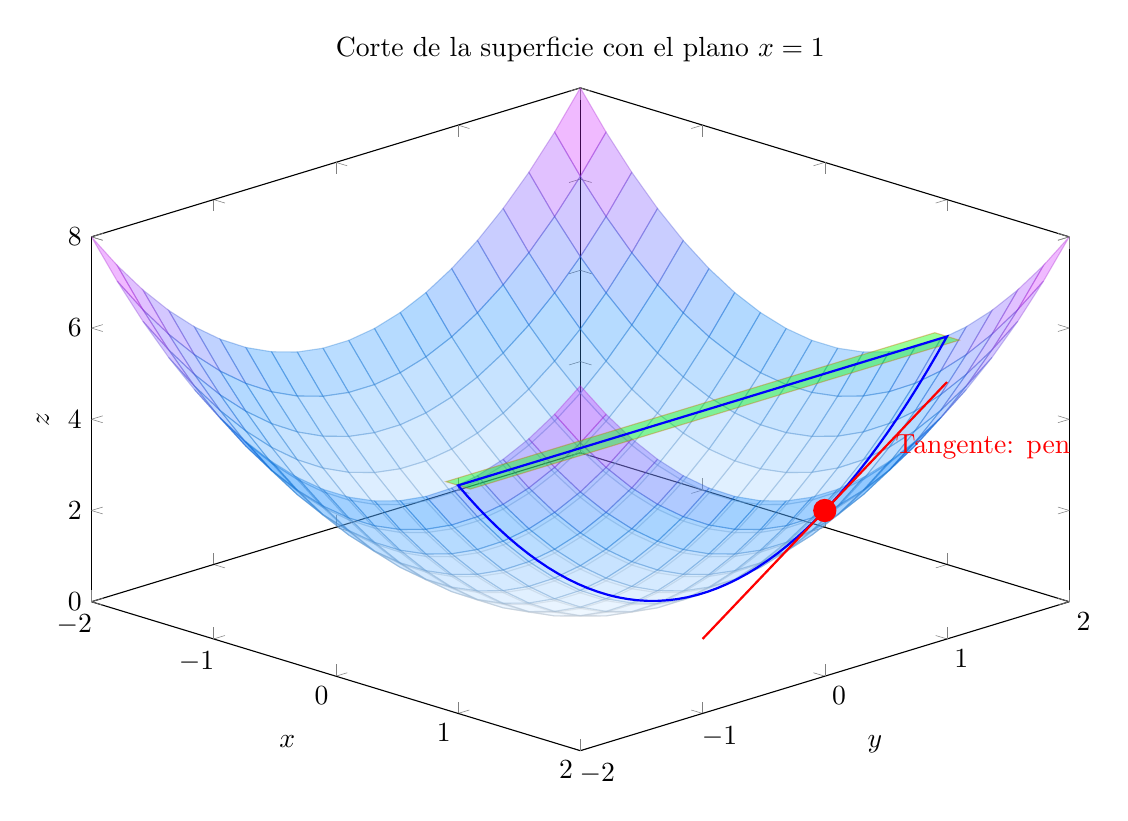
\begin{tikzpicture}
  \begin{axis}[
      view={45}{30},
      width=14cm, height=10cm,
      xlabel={$x$}, ylabel={$y$}, zlabel={$z$},
      xmin=-2, xmax=2, ymin=-2, ymax=2, zmin=0, zmax=8,
      title={Corte de la superficie con el plano \(x=1\)}
  ]
    % Superficie translúcida
    \addplot3[surf,opacity=0.3,colormap/cool,domain=-2:2, y domain=-2:2,samples=20] {x^2 + y^2};
    
    % Plano x=1
    \addplot3[surf,opacity=0.4,color=green,domain=0.9:1.1,y domain=-2:2,samples=2] {1 + y^2};
    
    % Curva de intersección x=1
    \addplot3[thick,color=blue,domain=-2:2,samples=50] (1,x,{1 + x^2});
    
    % Punto de tangencia
    \addplot3[only marks, mark=*, mark size=4pt, color=red] coordinates {(1,1,2)};
    
    % Recta tangente con pendiente 2
    \addplot3[thick,color=red,domain=0:2,samples=2] (1,x,{2*(x-1) + 2});
    
    \node[anchor=west] at (axis cs:1,1.5,3) {\textcolor{red}{Tangente: pendiente = 2}};
  \end{axis}
\end{tikzpicture}
\caption{Curva azul: intersección con \(x=1\). Recta roja: tangente con pendiente \(\frac{\partial f}{\partial y} = 2\).}
\label{fig:corte_y}
\end{figure}

\paragraph{Ejemplo 2: Silla de montar (Paraboloide hiperbólico).}

Consideremos ahora \(f(x,y) = x^2 - y^2\), una superficie con forma de silla de montar.

Calculamos las derivadas parciales:
\[
\frac{\partial f}{\partial x} = 2x, \quad \frac{\partial f}{\partial y} = -2y
\]

En el punto \((1, 1, 0)\):
\[
\frac{\partial f}{\partial x}\bigg|_{(1,1)} = 2, \quad \frac{\partial f}{\partial y}\bigg|_{(1,1)} = -2
\]

\begin{figure}[h!]
\centering
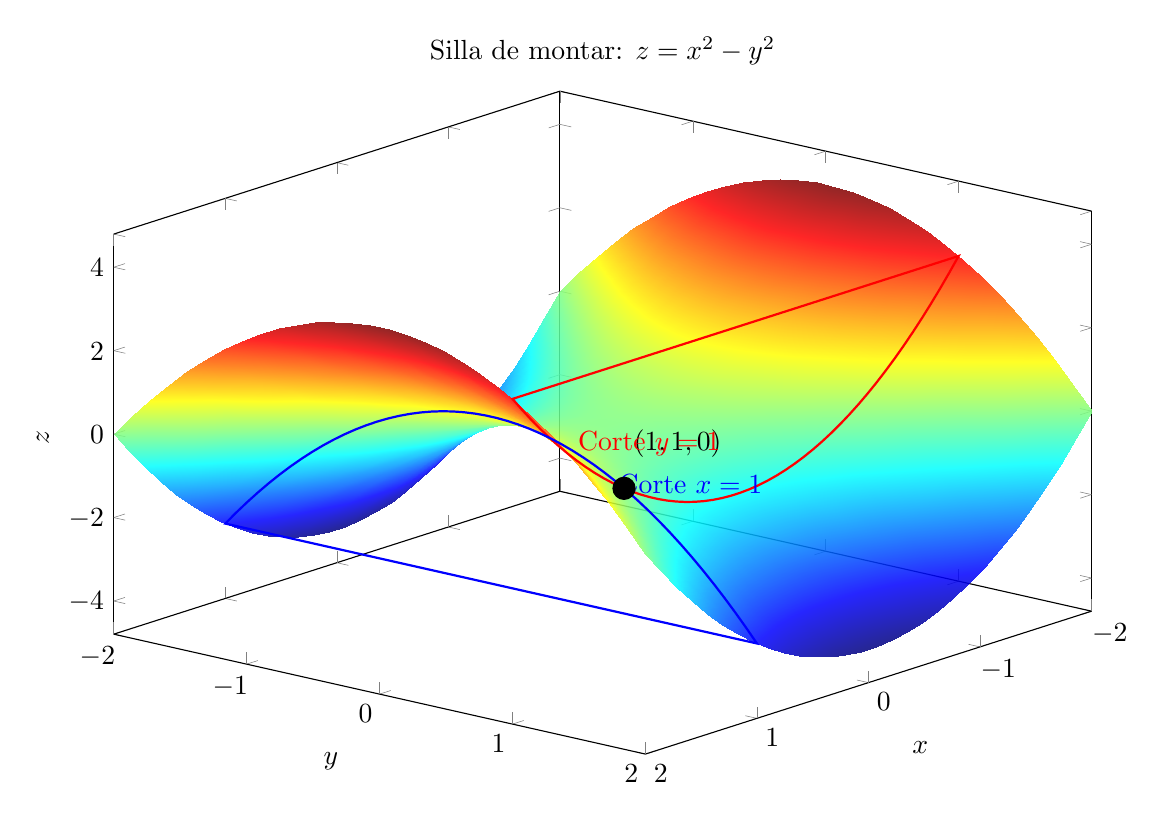
\begin{tikzpicture}
  \begin{axis}[
      view={130}{25},
      width=14cm, height=10cm,
      xlabel={$x$}, ylabel={$y$}, zlabel={$z$},
      domain=-2:2, y domain=-2:2,
      samples=30, samples y=30,
      colormap/jet,
      title={Silla de montar: \(z = x^2 - y^2\)}
  ]
    % Superficie
    \addplot3[surf,opacity=0.85,shader=interp] {x^2 - y^2};
    
    % Punto de interés
    \addplot3[only marks, mark=*, mark size=4pt, color=black] coordinates {(1,1,0)};
    \node[anchor=south west] at (axis cs:1,1,0.5) {$(1,1,0)$};
    
    % Curvas de corte
    \addplot3[thick,color=red,domain=-2:2,samples=50] (x,1,{x^2 - 1});
    \addplot3[thick,color=blue,domain=-2:2,samples=50] (1,x,{1 - x^2});
    
    % Etiquetas de las curvas
    \node[anchor=west,red] at (axis cs:1.5,1,1.5) {Corte $y=1$};
    \node[anchor=south,blue] at (axis cs:1,1.5,0) {Corte $x=1$};
  \end{axis}
\end{tikzpicture}
\caption{Silla de montar con cortes que muestran pendientes opuestas en direcciones perpendiculares.}
\label{fig:silla_montar}
\end{figure}

\paragraph{Comparación visual de curvaturas.}

La siguiente gráfica muestra las curvas de nivel de la función paraboloide. Cada círculo representa puntos donde la función tiene el mismo valor:

\begin{figure}[h!]
\centering
\begin{tikzpicture}
  \begin{axis}[
      axis equal image,
      width=12cm,height=10cm,
      axis lines=middle, xlabel={$x$}, ylabel={$y$},
      xmin=-2.5, xmax=2.5, ymin=-2.5, ymax=2.5,
      grid=both, grid style={gray!20},
      title={Curvas de nivel de \(f(x,y) = x^2 + y^2\)}
  ]
    % Curvas de nivel (círculos concéntricos)
    \addplot[brand,thick,domain=0:360,samples=100] ({cos(x)},{sin(x)});
    \addplot[brand,thick,domain=0:360,samples=100] ({1.414*cos(x)},{1.414*sin(x)});
    \addplot[brand,thick,domain=0:360,samples=100] ({1.732*cos(x)},{1.732*sin(x)});
    \addplot[brand,thick,domain=0:360,samples=100] ({2*cos(x)},{2*sin(x)});
    
    % Puntos de referencia
    \addplot[only marks,mark=*,mark size=3pt,color=red] coordinates {(1,0) (0,1) (1,1)};
    
    % Etiquetas de los puntos
    \node[anchor=west] at (axis cs:1.1,0) {$(1,0)$};
    \node[anchor=south] at (axis cs:0,1.1) {$(0,1)$};
    \node[anchor=south west] at (axis cs:1.1,1.1) {$(1,1)$};
  \end{axis}
\end{tikzpicture}
\caption{Curvas de nivel: círculos concéntricos para $k=1,2,3,4$.}
\label{fig:nivel_vectores}
\end{figure}

\paragraph{Interpretación práctica con software.}

En software como \textbf{GeoGebra}, \textbf{Mathematica}, \textbf{MATLAB} o \textbf{Python} (matplotlib), podemos:

\begin{enumerate}
  \item \textbf{Graficar la superficie} \(z = f(x,y)\) en 3D
  \item \textbf{Crear planos de corte} \(x = x_0\) o \(y = y_0\)
  \item \textbf{Visualizar las curvas de intersección}
  \item \textbf{Calcular y dibujar las rectas tangentes} con pendientes dadas por las derivadas parciales
  \item \textbf{Animar} el movimiento del punto para ver cómo cambian las pendientes
\end{enumerate}

\begin{InfoBox}
\Meta{Herramientas recomendadas}{GeoGebra 3D, Desmos 3D Calculator, Python (matplotlib + numpy), MATLAB, Mathematica, Wolfram Alpha}

\Meta{Ventajas de la visualización}{Permite comprender intuitivamente conceptos abstractos, verificar cálculos analíticos y explorar comportamientos locales de funciones complejas.}
\end{InfoBox}

\paragraph{Ejercicio guiado con visualización.}

\begin{EjercicioBox}[Ejercicio: Cono]
Considera la función \(f(x,y) = \sqrt{x^2 + y^2}\), que representa un cono.

\textbf{Tareas:}
\begin{enumerate}
  \item Calcula \(\frac{\partial f}{\partial x}\) y \(\frac{\partial f}{\partial y}\)
  \item Evalúa las derivadas en el punto \((3, 4)\)
  \item Interpreta geométricamente el resultado
\end{enumerate}

\textbf{Solución:}

\textbf{1. Cálculo de derivadas parciales:}
\begin{align*}
\frac{\partial f}{\partial x} &= \frac{\partial}{\partial x}\sqrt{x^2 + y^2} = \frac{x}{\sqrt{x^2 + y^2}} = \frac{x}{f(x,y)} \\[0.5em]
\frac{\partial f}{\partial y} &= \frac{\partial}{\partial y}\sqrt{x^2 + y^2} = \frac{y}{\sqrt{x^2 + y^2}} = \frac{y}{f(x,y)}
\end{align*}

\textbf{2. Evaluación en} \((3,4)\):
\[
f(3,4) = \sqrt{9 + 16} = 5
\]
\[
\frac{\partial f}{\partial x}\bigg|_{(3,4)} = \frac{3}{5} = 0.6, \quad \frac{\partial f}{\partial y}\bigg|_{(3,4)} = \frac{4}{5} = 0.8
\]

\textbf{3. Interpretación geométrica:}
\begin{itemize}
  \item Al movernos en dirección \(x\) desde \((3,4,5)\), la superficie sube con pendiente 0.6
  \item Al movernos en dirección \(y\), la pendiente es 0.8
  \item Ambas pendientes son positivas porque nos alejamos del vértice del cono en el origen
\end{itemize}
\end{EjercicioBox}

\begin{figure}[h!]
\centering
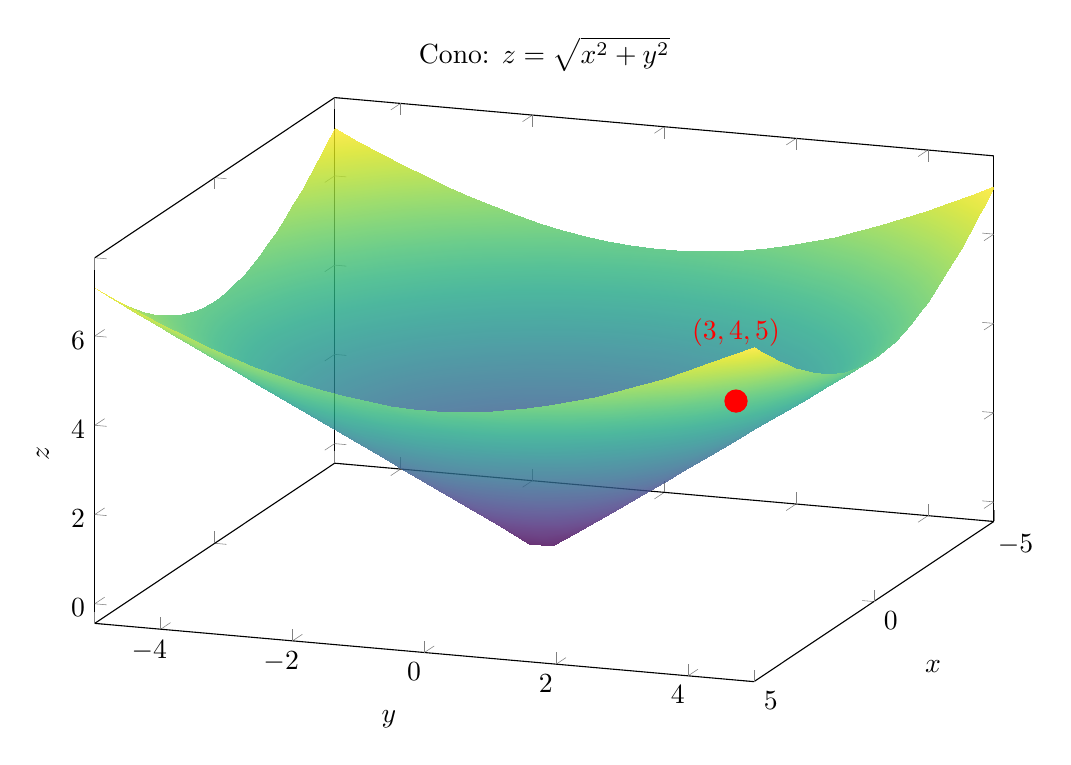
\begin{tikzpicture}
  \begin{axis}[
      view={110}{25},
      width=13cm, height=9cm,
      xlabel={$x$}, ylabel={$y$}, zlabel={$z$},
      domain=-5:5, y domain=-5:5,
      samples=30, samples y=30,
      colormap/viridis,
      title={Cono: \(z = \sqrt{x^2 + y^2}\)}
  ]
    % Superficie del cono
    \addplot3[surf,opacity=0.8,shader=interp] {sqrt(x^2 + y^2)};
    
    % Punto de interés (3,4,5)
    \addplot3[only marks, mark=*, mark size=4pt, color=red] coordinates {(3,4,5)};
    \node[anchor=south] at (axis cs:3,4,6) {\textcolor{red}{$(3,4,5)$}};
  \end{axis}
\end{tikzpicture}
\caption{Superficie cónica con punto de análisis en \((3,4,5)\).}
\label{fig:cono}
\end{figure}

\paragraph{Conclusión.}

La construcción geométrica de derivadas parciales nos permite:
\begin{itemize}
  \item \textbf{Visualizar} cómo una superficie cambia localmente en diferentes direcciones
  \item \textbf{Comprender} que cada derivada parcial es la pendiente de una curva específica
  \item \textbf{Utilizar software} para verificar y explorar cálculos analíticos
  \item \textbf{Desarrollar intuición} sobre el comportamiento de funciones multivariables
\end{itemize}

\subsubsection{Reglas de derivación parcial}

\begin{TemaBox}[Reglas de derivación: Extensión al caso multivariable]
Las reglas de derivación que conocemos del cálculo de una variable se extienden naturalmente a las derivadas parciales. La diferencia clave es que al derivar respecto a una variable, tratamos las demás como constantes.
\end{TemaBox}

\paragraph{Introducción.}
Las reglas de derivación parcial nos permiten calcular derivadas de funciones complejas de manera sistemática y eficiente. Estas reglas son idénticas a las del cálculo de una variable, pero aplicadas variable por variable.

\paragraph{Reglas básicas.}

Sea \(f(x,y)\) y \(g(x,y)\) funciones de dos variables, y \(c\) una constante.

\begin{InfoBox}
\Meta{Regla 1: Constante}{}
\[
\frac{\partial}{\partial x}(c) = 0, \quad \frac{\partial}{\partial y}(c) = 0
\]

\Meta{Regla 2: Constante por una función}{}
\[
\frac{\partial}{\partial x}[c \cdot f(x,y)] = c \cdot \frac{\partial f}{\partial x}
\]

\Meta{Regla 3: Suma y diferencia}{}
\[
\frac{\partial}{\partial x}[f(x,y) \pm g(x,y)] = \frac{\partial f}{\partial x} \pm \frac{\partial g}{\partial x}
\]

\Meta{Regla 4: Producto}{}
\[
\frac{\partial}{\partial x}[f(x,y) \cdot g(x,y)] = f \cdot \frac{\partial g}{\partial x} + g \cdot \frac{\partial f}{\partial x}
\]

\Meta{Regla 5: Cociente}{}
\[
\frac{\partial}{\partial x}\left[\frac{f(x,y)}{g(x,y)}\right] = \frac{g \cdot \frac{\partial f}{\partial x} - f \cdot \frac{\partial g}{\partial x}}{g^2}
\]

\Meta{Regla 6: Potencia}{}
\[
\frac{\partial}{\partial x}[f(x,y)]^n = n[f(x,y)]^{n-1} \cdot \frac{\partial f}{\partial x}
\]
\end{InfoBox}

\paragraph{Tabla resumen de derivadas parciales comunes.}

\begin{table}[h!]
\centering
\begin{tabular}{|c|c|c|}
\hline
\textbf{Función} & \(\boldsymbol{\frac{\partial f}{\partial x}}\) & \(\boldsymbol{\frac{\partial f}{\partial y}}\) \\
\hline
\(f(x,y) = x^n\) & \(nx^{n-1}\) & \(0\) \\
\hline
\(f(x,y) = y^n\) & \(0\) & \(ny^{n-1}\) \\
\hline
\(f(x,y) = x^n y^m\) & \(nx^{n-1}y^m\) & \(mx^n y^{m-1}\) \\
\hline
\(f(x,y) = e^x\) & \(e^x\) & \(0\) \\
\hline
\(f(x,y) = e^{xy}\) & \(ye^{xy}\) & \(xe^{xy}\) \\
\hline
\(f(x,y) = \ln(x)\) & \(\frac{1}{x}\) & \(0\) \\
\hline
\(f(x,y) = \ln(xy)\) & \(\frac{1}{x}\) & \(\frac{1}{y}\) \\
\hline
\(f(x,y) = \sin(x)\) & \(\cos(x)\) & \(0\) \\
\hline
\(f(x,y) = \sin(xy)\) & \(y\cos(xy)\) & \(x\cos(xy)\) \\
\hline
\(f(x,y) = \cos(x)\) & \(-\sin(x)\) & \(0\) \\
\hline
\(f(x,y) = \tan(x)\) & \(\sec^2(x)\) & \(0\) \\
\hline
\end{tabular}
\caption{Derivadas parciales de funciones comunes.}
\label{tab:derivadas_comunes}
\end{table}

\paragraph{Ejemplos resueltos detallados.}

\begin{EjercicioBox}[Ejemplo 1: Regla de la suma y producto]
Calcular las derivadas parciales de:
\[
f(x,y) = 3x^2y + 5xy^3 - 7x + 2y
\]

\textbf{Solución:}

\textbf{Para} \(\frac{\partial f}{\partial x}\): Derivamos término por término respecto a \(x\)

\begin{align*}
\frac{\partial f}{\partial x} &= \frac{\partial}{\partial x}(3x^2y) + \frac{\partial}{\partial x}(5xy^3) - \frac{\partial}{\partial x}(7x) + \frac{\partial}{\partial x}(2y) \\
&= 3y \cdot 2x + 5y^3 \cdot 1 - 7 + 0 \\
&= \boxed{6xy + 5y^3 - 7}
\end{align*}

\textbf{Para} \(\frac{\partial f}{\partial y}\): Derivamos término por término respecto a \(y\)

\begin{align*}
\frac{\partial f}{\partial y} &= \frac{\partial}{\partial y}(3x^2y) + \frac{\partial}{\partial y}(5xy^3) - \frac{\partial}{\partial y}(7x) + \frac{\partial}{\partial y}(2y) \\
&= 3x^2 \cdot 1 + 5x \cdot 3y^2 - 0 + 2 \\
&= \boxed{3x^2 + 15xy^2 + 2}
\end{align*}
\end{EjercicioBox}

\begin{EjercicioBox}[Ejemplo 2: Regla del producto]
Calcular las derivadas parciales de:
\[
f(x,y) = (x^2 + y)(3x - y^2)
\]

\textbf{Solución:}

\textbf{Para} \(\frac{\partial f}{\partial x}\): Usamos la regla del producto

Sean \(u = x^2 + y\) y \(v = 3x - y^2\)

\begin{align*}
\frac{\partial f}{\partial x} &= u \cdot \frac{\partial v}{\partial x} + v \cdot \frac{\partial u}{\partial x} \\
&= (x^2 + y) \cdot 3 + (3x - y^2) \cdot 2x \\
&= 3x^2 + 3y + 6x^2 - 2xy^2 \\
&= \boxed{9x^2 - 2xy^2 + 3y}
\end{align*}

\textbf{Para} \(\frac{\partial f}{\partial y}\):

\begin{align*}
\frac{\partial f}{\partial y} &= u \cdot \frac{\partial v}{\partial y} + v \cdot \frac{\partial u}{\partial y} \\
&= (x^2 + y) \cdot (-2y) + (3x - y^2) \cdot 1 \\
&= -2x^2y - 2y^2 + 3x - y^2 \\
&= \boxed{-2x^2y - 3y^2 + 3x}
\end{align*}
\end{EjercicioBox}

\begin{EjercicioBox}[Ejemplo 3: Regla del cociente]
Calcular las derivadas parciales de:
\[
f(x,y) = \frac{x^2 + y}{x - 2y}
\]

\textbf{Solución:}

Sean \(u = x^2 + y\) y \(v = x - 2y\)

\textbf{Para} \(\frac{\partial f}{\partial x}\): Aplicamos la regla del cociente

\begin{align*}
\frac{\partial f}{\partial x} &= \frac{v \cdot \frac{\partial u}{\partial x} - u \cdot \frac{\partial v}{\partial x}}{v^2} \\
&= \frac{(x - 2y) \cdot 2x - (x^2 + y) \cdot 1}{(x - 2y)^2} \\
&= \frac{2x^2 - 4xy - x^2 - y}{(x - 2y)^2} \\
&= \boxed{\frac{x^2 - 4xy - y}{(x - 2y)^2}}
\end{align*}

\textbf{Para} \(\frac{\partial f}{\partial y}\):

\begin{align*}
\frac{\partial f}{\partial y} &= \frac{v \cdot \frac{\partial u}{\partial y} - u \cdot \frac{\partial v}{\partial y}}{v^2} \\
&= \frac{(x - 2y) \cdot 1 - (x^2 + y) \cdot (-2)}{(x - 2y)^2} \\
&= \frac{x - 2y + 2x^2 + 2y}{(x - 2y)^2} \\
&= \boxed{\frac{2x^2 + x}{(x - 2y)^2}}
\end{align*}
\end{EjercicioBox}

\begin{EjercicioBox}[Ejemplo 4: Regla de la potencia (cadena)]
Calcular las derivadas parciales de:
\[
f(x,y) = (x^3 + xy^2)^5
\]

\textbf{Solución:}

Sea \(u = x^3 + xy^2\), entonces \(f = u^5\)

\textbf{Para} \(\frac{\partial f}{\partial x}\): Aplicamos la regla de la cadena

\begin{align*}
\frac{\partial f}{\partial x} &= 5u^4 \cdot \frac{\partial u}{\partial x} \\
&= 5(x^3 + xy^2)^4 \cdot (3x^2 + y^2) \\
&= \boxed{5(x^3 + xy^2)^4(3x^2 + y^2)}
\end{align*}

\textbf{Para} \(\frac{\partial f}{\partial y}\):

\begin{align*}
\frac{\partial f}{\partial y} &= 5u^4 \cdot \frac{\partial u}{\partial y} \\
&= 5(x^3 + xy^2)^4 \cdot (2xy) \\
&= \boxed{10xy(x^3 + xy^2)^4}
\end{align*}
\end{EjercicioBox}

\begin{EjercicioBox}[Ejemplo 5: Funciones exponenciales y trigonométricas]
Calcular las derivadas parciales de:
\[
f(x,y) = e^{x^2y} \sin(xy)
\]

\textbf{Solución:}

Usamos la regla del producto: \(f = e^{x^2y} \cdot \sin(xy)\)

\textbf{Para} \(\frac{\partial f}{\partial x}\):

\begin{align*}
\frac{\partial f}{\partial x} &= e^{x^2y} \cdot \frac{\partial}{\partial x}[\sin(xy)] + \sin(xy) \cdot \frac{\partial}{\partial x}[e^{x^2y}] \\
&= e^{x^2y} \cdot \cos(xy) \cdot y + \sin(xy) \cdot e^{x^2y} \cdot 2xy \\
&= e^{x^2y}[y\cos(xy) + 2xy\sin(xy)] \\
&= \boxed{ye^{x^2y}[\cos(xy) + 2x\sin(xy)]}
\end{align*}

\textbf{Para} \(\frac{\partial f}{\partial y}\):

\begin{align*}
\frac{\partial f}{\partial y} &= e^{x^2y} \cdot \frac{\partial}{\partial y}[\sin(xy)] + \sin(xy) \cdot \frac{\partial}{\partial y}[e^{x^2y}] \\
&= e^{x^2y} \cdot \cos(xy) \cdot x + \sin(xy) \cdot e^{x^2y} \cdot x^2 \\
&= xe^{x^2y}[\cos(xy) + x\sin(xy)] \\
&= \boxed{xe^{x^2y}[\cos(xy) + x\sin(xy)]}
\end{align*}
\end{EjercicioBox}

\begin{EjercicioBox}[Ejemplo 6: Función logarítmica]
Calcular las derivadas parciales de:
\[
f(x,y) = \ln(x^2 + y^2 + 1)
\]

\textbf{Solución:}

Sea \(u = x^2 + y^2 + 1\), entonces \(f = \ln(u)\)

\textbf{Para} \(\frac{\partial f}{\partial x}\): Usamos la regla de la cadena

\begin{align*}
\frac{\partial f}{\partial x} &= \frac{1}{u} \cdot \frac{\partial u}{\partial x} \\
&= \frac{1}{x^2 + y^2 + 1} \cdot 2x \\
&= \boxed{\frac{2x}{x^2 + y^2 + 1}}
\end{align*}

\textbf{Para} \(\frac{\partial f}{\partial y}\):

\begin{align*}
\frac{\partial f}{\partial y} &= \frac{1}{u} \cdot \frac{\partial u}{\partial y} \\
&= \frac{1}{x^2 + y^2 + 1} \cdot 2y \\
&= \boxed{\frac{2y}{x^2 + y^2 + 1}}
\end{align*}
\end{EjercicioBox}

\paragraph{Derivadas parciales de orden superior.}

Las derivadas parciales pueden derivarse nuevamente, obteniendo derivadas de segundo orden o superiores.

\begin{InfoBox}
\Meta{Notación}{Para \(f(x,y)\):}

\textbf{Segundas derivadas parciales:}
\begin{itemize}
  \item \(\frac{\partial^2 f}{\partial x^2} = f_{xx}\): derivar dos veces respecto a \(x\)
  \item \(\frac{\partial^2 f}{\partial y^2} = f_{yy}\): derivar dos veces respecto a \(y\)
  \item \(\frac{\partial^2 f}{\partial x \partial y} = f_{xy}\): derivar primero respecto a \(y\), luego respecto a \(x\)
  \item \(\frac{\partial^2 f}{\partial y \partial x} = f_{yx}\): derivar primero respecto a \(x\), luego respecto a \(y\)
\end{itemize}

\Meta{Teorema de Schwarz}{Si las derivadas parciales mixtas \(f_{xy}\) y \(f_{yx}\) son continuas, entonces:}
\[
\frac{\partial^2 f}{\partial x \partial y} = \frac{\partial^2 f}{\partial y \partial x}
\]
Es decir, el orden de derivación no importa.
\end{InfoBox}

\begin{EjercicioBox}[Ejemplo 7: Derivadas de segundo orden]
Calcular todas las segundas derivadas parciales de:
\[
f(x,y) = x^3y^2 + x^2y
\]

\textbf{Solución:}

\textbf{Primero calculamos las derivadas de primer orden:}
\begin{align*}
f_x &= 3x^2y^2 + 2xy \\
f_y &= 2x^3y + x^2
\end{align*}

\textbf{Ahora las segundas derivadas:}

\begin{align*}
f_{xx} &= \frac{\partial}{\partial x}(3x^2y^2 + 2xy) = \boxed{6xy^2 + 2y} \\[0.5em]
f_{yy} &= \frac{\partial}{\partial y}(2x^3y + x^2) = \boxed{2x^3} \\[0.5em]
f_{xy} &= \frac{\partial}{\partial y}(3x^2y^2 + 2xy) = \boxed{6x^2y + 2x} \\[0.5em]
f_{yx} &= \frac{\partial}{\partial x}(2x^3y + x^2) = \boxed{6x^2y + 2x}
\end{align*}

\textbf{Verificación:} Como esperábamos por el Teorema de Schwarz: \(f_{xy} = f_{yx}\)
\end{EjercicioBox}

\paragraph{Errores comunes al calcular derivadas parciales.}

\begin{itemize}
  \item \textbf{Error 1:} Olvidar que las otras variables son constantes.
  
  \textit{Incorrecto:} \(\frac{\partial}{\partial x}(xy^2) = y^2 + 2xy\)
  
  \textit{Correcto:} \(\frac{\partial}{\partial x}(xy^2) = y^2\) (porque \(y\) es constante)
  
  \item \textbf{Error 2:} Confundir el orden en derivadas mixtas.
  
  Para \(\frac{\partial^2 f}{\partial x \partial y}\): primero derivar respecto a \(y\), luego respecto a \(x\)
  
  \item \textbf{Error 3:} No aplicar la regla de la cadena cuando es necesaria.
  
  \textit{Incorrecto:} \(\frac{\partial}{\partial x}[\sin(x^2y)] = \cos(x^2y)\)
  
  \textit{Correcto:} \(\frac{\partial}{\partial x}[\sin(x^2y)] = \cos(x^2y) \cdot 2xy\)
\end{itemize}

\paragraph{Ejercicios propuestos.}

Calcular las derivadas parciales de las siguientes funciones:

\begin{enumerate}
  \item \(f(x,y) = 5x^4y^3 - 3x^2y + 7xy^2 - 2\)
  
  \item \(f(x,y) = \frac{x^3 - y^3}{x + y}\)
  
  \item \(f(x,y) = e^{x/y} + \ln(x^2 + y^2)\)
  
  \item \(f(x,y) = x^y\) \textit{(Sugerencia: \(x^y = e^{y\ln x}\))}
  
  \item \(f(x,y) = \cos(x^2 + y^2) \cdot e^{xy}\)
  
  \item \(f(x,y,z) = xyz + x^2y + y^2z + z^2x\) (tres variables)
  
  \item Calcular \(f_{xx}\), \(f_{yy}\), \(f_{xy}\) para \(f(x,y) = \sin(x)\cos(y)\)
  
  \item Verificar que \(f_{xy} = f_{yx}\) para \(f(x,y) = e^{xy^2}\)
\end{enumerate}

\subsubsection{Regla de la cadena para varias variables}

\begin{TemaBox}[Regla de la cadena: Composición de funciones multivariables]
La regla de la cadena para funciones de varias variables nos permite calcular derivadas cuando las variables son, a su vez, funciones de otras variables. Es una extensión natural de la regla de la cadena del cálculo de una variable y es fundamental en física, ingeniería y optimización.
\end{TemaBox}

\paragraph{Introducción.}
En cálculo de una variable, la regla de la cadena establece que si \(y = f(u)\) y \(u = g(x)\), entonces:
\[
\frac{dy}{dx} = \frac{dy}{du} \cdot \frac{du}{dx}
\]

Para funciones de varias variables, esta regla se extiende considerando todas las trayectorias de dependencia entre variables.

\paragraph{Caso 1: Función de dos variables con dependencia de una sola variable.}

\begin{InfoBox}
\Meta{Teorema (Regla de la cadena - Caso 1)}{Sea \(z = f(x,y)\) una función diferenciable de \(x\) e \(y\), donde:}
\begin{itemize}
  \item \(x = x(t)\)
  \item \(y = y(t)\)
\end{itemize}

Entonces la \textbf{derivada total} de \(z\) respecto a \(t\) es:
\[
\frac{dz}{dt} = \frac{\partial z}{\partial x} \cdot \frac{dx}{dt} + \frac{\partial z}{\partial y} \cdot \frac{dy}{dt}
\]

\Meta{Interpretación}{La tasa de cambio de \(z\) respecto a \(t\) se obtiene sumando las contribuciones de cada variable intermedia.}
\end{InfoBox}

\paragraph{Visualización de las dependencias.}

Para visualizar la regla de la cadena, imaginamos un diagrama de árbol con las siguientes dependencias:

\begin{InfoBox}
\Meta{Caminos de dependencia}{Existen dos caminos desde \(t\) hasta \(z\):}
\begin{itemize}
  \item \textbf{Camino 1:} \(t \to x \to z\) contribuye: \(\frac{\partial z}{\partial x} \cdot \frac{dx}{dt}\)
  \item \textbf{Camino 2:} \(t \to y \to z\) contribuye: \(\frac{\partial z}{\partial y} \cdot \frac{dy}{dt}\)
\end{itemize}

La derivada total es la suma de las contribuciones de ambos caminos.
\end{InfoBox}

\begin{EjercicioBox}[Ejemplo 1: Caso básico]
Sea \(z = x^2 + xy + y^2\) donde \(x = t^2\) y \(y = t^3\). Calcular \(\frac{dz}{dt}\).

\textbf{Solución:}

\textbf{Método 1: Aplicando la regla de la cadena}

Primero calculamos las derivadas parciales de \(z\):
\begin{align*}
\frac{\partial z}{\partial x} &= 2x + y \\
\frac{\partial z}{\partial y} &= x + 2y
\end{align*}

Luego las derivadas de \(x\) e \(y\) respecto a \(t\):
\begin{align*}
\frac{dx}{dt} &= 2t \\
\frac{dy}{dt} &= 3t^2
\end{align*}

Aplicamos la regla de la cadena:
\begin{align*}
\frac{dz}{dt} &= \frac{\partial z}{\partial x} \cdot \frac{dx}{dt} + \frac{\partial z}{\partial y} \cdot \frac{dy}{dt} \\
&= (2x + y)(2t) + (x + 2y)(3t^2) \\
&= (2t^2 + t^3)(2t) + (t^2 + 2t^3)(3t^2) \\
&= 4t^3 + 2t^4 + 3t^4 + 6t^5 \\
&= \boxed{6t^5 + 5t^4 + 4t^3}
\end{align*}

\textbf{Método 2: Sustitución directa (verificación)}

Sustituimos \(x = t^2\) y \(y = t^3\) en \(z\):
\begin{align*}
z &= (t^2)^2 + (t^2)(t^3) + (t^3)^2 \\
&= t^4 + t^5 + t^6
\end{align*}

Derivamos directamente:
\[
\frac{dz}{dt} = 4t^3 + 5t^4 + 6t^5 = \boxed{6t^5 + 5t^4 + 4t^3}
\]

\textbf{Ambos métodos dan el mismo resultado.}
\end{EjercicioBox}

\begin{EjercicioBox}[Ejemplo 2: Funciones trigonométricas]
Sea \(z = e^x \sin(y)\) donde \(x = t^2\) y \(y = \pi t\). Calcular \(\frac{dz}{dt}\) cuando \(t = 1\).

\textbf{Solución:}

Calculamos las derivadas parciales:
\begin{align*}
\frac{\partial z}{\partial x} &= e^x \sin(y) \\
\frac{\partial z}{\partial y} &= e^x \cos(y)
\end{align*}

Las derivadas respecto a \(t\):
\begin{align*}
\frac{dx}{dt} &= 2t \\
\frac{dy}{dt} &= \pi
\end{align*}

Aplicamos la regla de la cadena:
\begin{align*}
\frac{dz}{dt} &= e^x \sin(y) \cdot 2t + e^x \cos(y) \cdot \pi \\
&= e^{t^2}[\sin(\pi t) \cdot 2t + \cos(\pi t) \cdot \pi]
\end{align*}

Evaluamos en \(t = 1\):
\begin{align*}
\frac{dz}{dt}\bigg|_{t=1} &= e^{1}[\sin(\pi) \cdot 2 + \cos(\pi) \cdot \pi] \\
&= e[0 \cdot 2 + (-1) \cdot \pi] \\
&= \boxed{-\pi e}
\end{align*}
\end{EjercicioBox}

\paragraph{Caso 2: Función de dos variables con dependencia de dos variables.}

\begin{InfoBox}
\Meta{Teorema (Regla de la cadena - Caso 2)}{Sea \(z = f(x,y)\) donde:}
\begin{itemize}
  \item \(x = x(u,v)\)
  \item \(y = y(u,v)\)
\end{itemize}

Entonces:
\[
\frac{\partial z}{\partial u} = \frac{\partial z}{\partial x} \cdot \frac{\partial x}{\partial u} + \frac{\partial z}{\partial y} \cdot \frac{\partial y}{\partial u}
\]

\[
\frac{\partial z}{\partial v} = \frac{\partial z}{\partial x} \cdot \frac{\partial x}{\partial v} + \frac{\partial z}{\partial y} \cdot \frac{\partial y}{\partial v}
\]
\end{InfoBox}

\paragraph{Visualización para el Caso 2.}

Para este caso más complejo, existen cuatro caminos desde las variables \(u\) y \(v\) hasta \(z\):

\begin{InfoBox}
\Meta{Caminos de dependencia para el Caso 2}{Cuatro caminos:}
\begin{itemize}
  \item \textbf{Camino 1:} \(u \to x \to z\) contribuye: \(\frac{\partial z}{\partial x} \cdot \frac{\partial x}{\partial u}\)
  \item \textbf{Camino 2:} \(u \to y \to z\) contribuye: \(\frac{\partial z}{\partial y} \cdot \frac{\partial y}{\partial u}\)
  \item \textbf{Camino 3:} \(v \to x \to z\) contribuye: \(\frac{\partial z}{\partial x} \cdot \frac{\partial x}{\partial v}\)
  \item \textbf{Camino 4:} \(v \to y \to z\) contribuye: \(\frac{\partial z}{\partial y} \cdot \frac{\partial y}{\partial v}\)
\end{itemize}

Por tanto:
\begin{align*}
\frac{\partial z}{\partial u} &= \frac{\partial z}{\partial x}\frac{\partial x}{\partial u} + \frac{\partial z}{\partial y}\frac{\partial y}{\partial u} \\
\frac{\partial z}{\partial v} &= \frac{\partial z}{\partial x}\frac{\partial x}{\partial v} + \frac{\partial z}{\partial y}\frac{\partial y}{\partial v}
\end{align*}
\end{InfoBox}

\begin{EjercicioBox}[Ejemplo 3: Coordenadas polares]
Sea \(z = x^2 + y^2\) donde \(x = r\cos(\theta)\) y \(y = r\sin(\theta)\). Calcular \(\frac{\partial z}{\partial r}\) y \(\frac{\partial z}{\partial \theta}\).

\textbf{Solución:}

Calculamos las derivadas parciales de \(z\):
\begin{align*}
\frac{\partial z}{\partial x} &= 2x \\
\frac{\partial z}{\partial y} &= 2y
\end{align*}

Las derivadas de \(x\) e \(y\) respecto a \(r\) y \(\theta\):
\begin{align*}
\frac{\partial x}{\partial r} &= \cos(\theta), \quad \frac{\partial x}{\partial \theta} = -r\sin(\theta) \\
\frac{\partial y}{\partial r} &= \sin(\theta), \quad \frac{\partial y}{\partial \theta} = r\cos(\theta)
\end{align*}

\textbf{Para} \(\frac{\partial z}{\partial r}\):
\begin{align*}
\frac{\partial z}{\partial r} &= \frac{\partial z}{\partial x} \cdot \frac{\partial x}{\partial r} + \frac{\partial z}{\partial y} \cdot \frac{\partial y}{\partial r} \\
&= 2x \cdot \cos(\theta) + 2y \cdot \sin(\theta) \\
&= 2r\cos^2(\theta) + 2r\sin^2(\theta) \\
&= 2r(\cos^2(\theta) + \sin^2(\theta)) \\
&= \boxed{2r}
\end{align*}

\textbf{Para} \(\frac{\partial z}{\partial \theta}\):
\begin{align*}
\frac{\partial z}{\partial \theta} &= \frac{\partial z}{\partial x} \cdot \frac{\partial x}{\partial \theta} + \frac{\partial z}{\partial y} \cdot \frac{\partial y}{\partial \theta} \\
&= 2x \cdot (-r\sin(\theta)) + 2y \cdot r\cos(\theta) \\
&= -2r^2\cos(\theta)\sin(\theta) + 2r^2\sin(\theta)\cos(\theta) \\
&= \boxed{0}
\end{align*}

\textbf{Interpretación:} \(\frac{\partial z}{\partial r} = 2r\) indica que \(z\) crece linealmente con \(r\). \(\frac{\partial z}{\partial \theta} = 0\) confirma que \(z = x^2 + y^2\) no depende del ángulo (es simétrica circularmente).
\end{EjercicioBox}

\begin{EjercicioBox}[Ejemplo 4: Caso general]
Sea \(z = x^2y + xy^2\) donde \(x = uv\) y \(y = u - v\). Calcular \(\frac{\partial z}{\partial u}\) y \(\frac{\partial z}{\partial v}\).

\textbf{Solución:}

Derivadas parciales de \(z\):
\begin{align*}
\frac{\partial z}{\partial x} &= 2xy + y^2 \\
\frac{\partial z}{\partial y} &= x^2 + 2xy
\end{align*}

Derivadas de \(x\) e \(y\):
\begin{align*}
\frac{\partial x}{\partial u} &= v, \quad \frac{\partial x}{\partial v} = u \\
\frac{\partial y}{\partial u} &= 1, \quad \frac{\partial y}{\partial v} = -1
\end{align*}

\textbf{Para} \(\frac{\partial z}{\partial u}\):
\begin{align*}
\frac{\partial z}{\partial u} &= (2xy + y^2) \cdot v + (x^2 + 2xy) \cdot 1 \\
&= v(2xy + y^2) + x^2 + 2xy
\end{align*}

Sustituyendo \(x = uv\) y \(y = u - v\):
\begin{align*}
\frac{\partial z}{\partial u} &= v[2uv(u-v) + (u-v)^2] + (uv)^2 + 2uv(u-v) \\
&= 2u v^2(u-v) + v(u-v)^2 + u^2v^2 + 2uv(u-v) \\
&= \boxed{2u^2v^2 - 2uv^3 + u^2v - 2uv^2 + v^3 + u^2v^2 + 2u^2v - 2uv^2}
\end{align*}

Simplificando:
\[
\frac{\partial z}{\partial u} = \boxed{3u^2v^2 + 2u^2v + u^2v - 4uv^2 + v^3}
\]

\textbf{Para} \(\frac{\partial z}{\partial v}\):
\begin{align*}
\frac{\partial z}{\partial v} &= (2xy + y^2) \cdot u + (x^2 + 2xy) \cdot (-1) \\
&= u(2xy + y^2) - x^2 - 2xy
\end{align*}

(Se puede desarrollar de manera similar sustituyendo valores)
\end{EjercicioBox}

\paragraph{Caso 3: Derivada implícita.}

Cuando tenemos una ecuación implícita \(F(x,y) = 0\), podemos usar la regla de la cadena para encontrar \(\frac{dy}{dx}\).

\begin{InfoBox}
\Meta{Derivación implícita}{Para \(F(x,y) = 0\):}
\[
\frac{dy}{dx} = -\frac{\frac{\partial F}{\partial x}}{\frac{\partial F}{\partial y}}
\]

\Meta{Generalización}{Para \(F(x,y,z) = 0\):}
\[
\frac{\partial z}{\partial x} = -\frac{\frac{\partial F}{\partial x}}{\frac{\partial F}{\partial z}}, \quad
\frac{\partial z}{\partial y} = -\frac{\frac{\partial F}{\partial y}}{\frac{\partial F}{\partial z}}
\]
\end{InfoBox}

\begin{EjercicioBox}[Ejemplo 5: Derivación implícita]
Para la ecuación \(x^3 + y^3 + xyz = 10\), calcular \(\frac{\partial z}{\partial x}\) y \(\frac{\partial z}{\partial y}\).

\textbf{Solución:}

Sea \(F(x,y,z) = x^3 + y^3 + xyz - 10\)

Calculamos las derivadas parciales de \(F\):
\begin{align*}
\frac{\partial F}{\partial x} &= 3x^2 + yz \\
\frac{\partial F}{\partial y} &= 3y^2 + xz \\
\frac{\partial F}{\partial z} &= xy
\end{align*}

Aplicamos la fórmula:
\[
\frac{\partial z}{\partial x} = -\frac{3x^2 + yz}{xy} = \boxed{-\frac{3x^2 + yz}{xy}}
\]

\[
\frac{\partial z}{\partial y} = -\frac{3y^2 + xz}{xy} = \boxed{-\frac{3y^2 + xz}{xy}}
\]
\end{EjercicioBox}

\paragraph{Aplicaciones prácticas.}

\begin{enumerate}
  \item \textbf{Física:} Cambio de coordenadas (cartesianas a polares, cilíndricas, esféricas)
  \item \textbf{Termodinámica:} Relaciones entre variables de estado
  \item \textbf{Optimización:} Funciones objetivo con restricciones paramétricas
  \item \textbf{Ingeniería:} Análisis de sensibilidad en sistemas complejos
  \item \textbf{Cinemática:} Velocidad y aceleración en trayectorias curvas
\end{enumerate}

\paragraph{Ejercicios propuestos.}

\begin{enumerate}
  \item Sea \(z = x^2 - y^2\) donde \(x = e^t\) y \(y = e^{-t}\). Calcular \(\frac{dz}{dt}\).
  
  \item Sea \(w = xyz\) donde \(x = t\), \(y = t^2\), \(z = t^3\). Calcular \(\frac{dw}{dt}\) cuando \(t = 2\).
  
  \item Sea \(z = \ln(x^2 + y^2)\) donde \(x = r\cos(\theta)\) y \(y = r\sin(\theta)\). Calcular \(\frac{\partial z}{\partial r}\) y \(\frac{\partial z}{\partial \theta}\).
  
  \item Sea \(z = e^{x+y}\) donde \(x = u^2 - v^2\) y \(y = 2uv\). Calcular \(\frac{\partial z}{\partial u}\) y \(\frac{\partial z}{\partial v}\).
  
  \item Para la ecuación implícita \(x^2 + y^2 + z^2 = 25\), calcular \(\frac{\partial z}{\partial x}\) y \(\frac{\partial z}{\partial y}\).
  
  \item Sea \(w = f(x,y,z)\) donde \(x = r\sin(\phi)\cos(\theta)\), \(y = r\sin(\phi)\sin(\theta)\), \(z = r\cos(\phi)\) (coordenadas esféricas). Expresar \(\frac{\partial w}{\partial r}\) usando la regla de la cadena.
  
  \item Verificar que si \(z = f(x-y, y-x)\), entonces \(\frac{\partial z}{\partial x} + \frac{\partial z}{\partial y} = 0\).
\end{enumerate}

\paragraph{Resumen de la regla de la cadena.}

\begin{table}[h!]
\centering
\begin{tabular}{|l|l|}
\hline
\textbf{Caso} & \textbf{Fórmula} \\
\hline
\(z = f(x,y)\), \(x=x(t)\), \(y=y(t)\) & \(\displaystyle \frac{dz}{dt} = \frac{\partial z}{\partial x}\frac{dx}{dt} + \frac{\partial z}{\partial y}\frac{dy}{dt}\) \\
\hline
\(z = f(x,y)\), \(x=x(u,v)\), \(y=y(u,v)\) & \(\displaystyle \frac{\partial z}{\partial u} = \frac{\partial z}{\partial x}\frac{\partial x}{\partial u} + \frac{\partial z}{\partial y}\frac{\partial y}{\partial u}\) \\
\hline
\(F(x,y,z) = 0\) & \(\displaystyle \frac{\partial z}{\partial x} = -\frac{\partial F/\partial x}{\partial F/\partial z}\) \\
\hline
\end{tabular}
\caption{Resumen de casos de la regla de la cadena.}
\label{tab:regla_cadena}
\end{table}

\subsection{Vector gradiente y derivada direccional}

\begin{TemaBox}[Vector gradiente y derivada direccional: Concepto unificador]
El gradiente es uno de los conceptos más importantes del cálculo multivariable. Unifica todas las derivadas parciales en un solo vector que apunta en la dirección de máximo crecimiento de la función. La derivada direccional nos permite medir la tasa de cambio en cualquier dirección deseada.
\end{TemaBox}

\paragraph{Introducción y contextualización.}

Hasta ahora hemos estudiado las derivadas parciales \(\frac{\partial f}{\partial x}\) y \(\frac{\partial f}{\partial y}\), que miden cómo cambia la función cuando nos movemos en las direcciones de los ejes coordenados. Pero, ¿qué sucede si queremos saber cómo cambia la función cuando nos movemos en cualquier otra dirección?

Imagina que estás de excursión en una montaña y tienes un mapa topográfico con curvas de nivel. Las derivadas parciales te dicen qué tan empinado es el terreno si caminas exactamente hacia el norte (\(y\)) o hacia el este (\(x\)). Pero si quieres caminar en dirección noreste, o en cualquier otra dirección, necesitas un concepto más general: \textbf{la derivada direccional}.

Además, si quieres encontrar la dirección más empinada para subir (o bajar) lo más rápido posible, necesitas el \textbf{vector gradiente}, que siempre apunta en la dirección de máxima pendiente ascendente.

\subsubsection{Cálculo e interpretación geométrica del gradiente y derivada direccional}

\paragraph{Definición: Vector gradiente.}

\begin{InfoBox}
\Meta{Definición}{Sea \(f(x,y)\) una función diferenciable. El \textbf{gradiente} de \(f\) se denota \(\nabla f\) (se lee "nabla \(f\)") y se define como:}
\[
\nabla f(x,y) = \left\langle \frac{\partial f}{\partial x}, \frac{\partial f}{\partial y} \right\rangle = \frac{\partial f}{\partial x}\mathbf{i} + \frac{\partial f}{\partial y}\mathbf{j}
\]

\Meta{Para funciones de tres variables}{\(f(x,y,z)\):}
\[
\nabla f(x,y,z) = \left\langle \frac{\partial f}{\partial x}, \frac{\partial f}{\partial y}, \frac{\partial f}{\partial z} \right\rangle
\]

\Meta{Notación alternativa}{También se escribe como \(\text{grad}\,f\).}
\end{InfoBox}

El gradiente es un \textbf{campo vectorial}: en cada punto \((x,y)\) del dominio de \(f\), el gradiente \(\nabla f(x,y)\) es un vector.

\paragraph{Propiedades geométricas del gradiente.}

El vector gradiente tiene propiedades geométricas fundamentales:

\begin{enumerate}
  \item \textbf{Dirección:} \(\nabla f\) apunta en la dirección de máximo crecimiento de \(f\).
  
  \item \textbf{Magnitud:} \(\|\nabla f\|\) es la razón de cambio máxima de \(f\) en ese punto.
  
  \item \textbf{Perpendicularidad:} \(\nabla f\) es perpendicular a las curvas de nivel de \(f\).
  
  \item \textbf{Cero en puntos críticos:} Si \(\nabla f = \mathbf{0}\), entonces \((x,y)\) es un punto crítico.
\end{enumerate}

\begin{EjercicioBox}[Ejemplo 1: Cálculo del gradiente]
Calcular el gradiente de \(f(x,y) = x^2 + xy + y^2\) y evaluarlo en el punto \((1,2)\).

\textbf{Solución:}

Calculamos las derivadas parciales:
\begin{align*}
\frac{\partial f}{\partial x} &= 2x + y \\
\frac{\partial f}{\partial y} &= x + 2y
\end{align*}

Por lo tanto, el gradiente es:
\[
\nabla f(x,y) = \langle 2x + y, x + 2y \rangle
\]

Evaluamos en \((1,2)\):
\[
\nabla f(1,2) = \langle 2(1) + 2, 1 + 2(2) \rangle = \langle 4, 5 \rangle
\]

\textbf{Interpretación:} En el punto \((1,2)\), la función crece más rápidamente en la dirección del vector \(\langle 4, 5 \rangle\), con una razón de cambio de \(\|\langle 4, 5 \rangle\| = \sqrt{16+25} = \sqrt{41} \approx 6.40\).
\end{EjercicioBox}

\begin{EjercicioBox}[Ejemplo 2: Gradiente de función exponencial]
Calcular \(\nabla f\) para \(f(x,y) = e^{x^2+y^2}\) en el punto \((0,0)\).

\textbf{Solución:}

\begin{align*}
\frac{\partial f}{\partial x} &= e^{x^2+y^2} \cdot 2x = 2xe^{x^2+y^2} \\
\frac{\partial f}{\partial y} &= e^{x^2+y^2} \cdot 2y = 2ye^{x^2+y^2}
\end{align*}

Por lo tanto:
\[
\nabla f(x,y) = \langle 2xe^{x^2+y^2}, 2ye^{x^2+y^2} \rangle
\]

En \((0,0)\):
\[
\nabla f(0,0) = \langle 2(0)e^{0}, 2(0)e^{0} \rangle = \langle 0, 0 \rangle
\]

\textbf{Interpretación:} El punto \((0,0)\) es un punto crítico (en este caso, un mínimo local).
\end{EjercicioBox}

\paragraph{Definición: Derivada direccional.}

Las derivadas parciales miden el cambio de \(f\) en las direcciones de los ejes. La derivada direccional generaliza esto a cualquier dirección.

\begin{InfoBox}
\Meta{Definición}{Sea \(f(x,y)\) una función diferenciable y \(\mathbf{u} = \langle a, b \rangle\) un \textbf{vector unitario} (es decir, \(\|\mathbf{u}\| = 1\)). La \textbf{derivada direccional} de \(f\) en la dirección de \(\mathbf{u}\) se denota \(D_{\mathbf{u}}f\) y se define como:}
\[
D_{\mathbf{u}}f(x,y) = \lim_{h \to 0} \frac{f(x + ha, y + hb) - f(x,y)}{h}
\]

\Meta{Fórmula práctica}{Si \(f\) es diferenciable:}
\[
D_{\mathbf{u}}f(x,y) = \nabla f(x,y) \cdot \mathbf{u} = \frac{\partial f}{\partial x}a + \frac{\partial f}{\partial y}b
\]

Esta fórmula nos dice que la derivada direccional es el producto punto entre el gradiente y el vector de dirección.
\end{InfoBox}

\paragraph{Relación entre gradiente y derivada direccional.}

La relación entre el gradiente y la derivada direccional es fundamental:

\begin{InfoBox}
\Meta{Teorema}{Sea \(f\) diferenciable y \(\mathbf{u}\) un vector unitario. Entonces:}
\[
D_{\mathbf{u}}f = \nabla f \cdot \mathbf{u} = \|\nabla f\| \|\mathbf{u}\| \cos(\theta) = \|\nabla f\| \cos(\theta)
\]
donde \(\theta\) es el ángulo entre \(\nabla f\) y \(\mathbf{u}\).

\Meta{Consecuencias importantes}{}
\begin{itemize}
  \item \textbf{Máximo:} \(D_{\mathbf{u}}f\) es máxima cuando \(\theta = 0\), es decir, cuando \(\mathbf{u}\) apunta en la dirección de \(\nabla f\). El valor máximo es \(\|\nabla f\|\).
  
  \item \textbf{Mínimo:} \(D_{\mathbf{u}}f\) es mínima cuando \(\theta = \pi\), es decir, cuando \(\mathbf{u}\) apunta en dirección opuesta a \(\nabla f\). El valor mínimo es \(-\|\nabla f\|\).
  
  \item \textbf{Cero:} \(D_{\mathbf{u}}f = 0\) cuando \(\theta = \pi/2\), es decir, cuando \(\mathbf{u}\) es perpendicular a \(\nabla f\). Esto ocurre en la dirección tangente a la curva de nivel.
\end{itemize}
\end{InfoBox}

\begin{EjercicioBox}[Ejemplo 3: Derivada direccional básica]
Sea \(f(x,y) = x^2 + y^2\). Calcular la derivada direccional en el punto \((3,4)\) en la dirección del vector \(\mathbf{v} = \langle 1, 1 \rangle\).

\textbf{Solución:}

\textbf{Paso 1:} Calcular el gradiente:
\begin{align*}
\frac{\partial f}{\partial x} &= 2x \\
\frac{\partial f}{\partial y} &= 2y
\end{align*}
\[
\nabla f(3,4) = \langle 2(3), 2(4) \rangle = \langle 6, 8 \rangle
\]

\textbf{Paso 2:} Normalizar el vector de dirección:
\[
\|\mathbf{v}\| = \sqrt{1^2 + 1^2} = \sqrt{2}
\]
\[
\mathbf{u} = \frac{\mathbf{v}}{\|\mathbf{v}\|} = \left\langle \frac{1}{\sqrt{2}}, \frac{1}{\sqrt{2}} \right\rangle
\]

\textbf{Paso 3:} Calcular la derivada direccional:
\begin{align*}
D_{\mathbf{u}}f(3,4) &= \nabla f(3,4) \cdot \mathbf{u} \\
&= \langle 6, 8 \rangle \cdot \left\langle \frac{1}{\sqrt{2}}, \frac{1}{\sqrt{2}} \right\rangle \\
&= \frac{6}{\sqrt{2}} + \frac{8}{\sqrt{2}} \\
&= \frac{14}{\sqrt{2}} = 7\sqrt{2} \approx \boxed{9.90}
\end{align*}

\textbf{Interpretación:} Si nos movemos desde \((3,4)\) en dirección \(45°\) (noreste), la función aumenta a una razón de aproximadamente \(9.90\) unidades por unidad de distancia.
\end{EjercicioBox}

\begin{EjercicioBox}[Ejemplo 4: Dirección de máximo crecimiento]
Para \(f(x,y) = x^2 - xy + y^2\) en el punto \((2,1)\):
\begin{enumerate}
  \item Encontrar la dirección de máximo crecimiento.
  \item Calcular la razón de cambio máxima.
  \item Encontrar la dirección de máximo decrecimiento.
\end{enumerate}

\textbf{Solución:}

\textbf{Calculamos el gradiente:}
\begin{align*}
\frac{\partial f}{\partial x} &= 2x - y \\
\frac{\partial f}{\partial y} &= -x + 2y
\end{align*}
\[
\nabla f(2,1) = \langle 2(2) - 1, -2 + 2(1) \rangle = \langle 3, 0 \rangle
\]

\textbf{a) Dirección de máximo crecimiento:}

El vector gradiente apunta en la dirección de máximo crecimiento. El vector unitario correspondiente es:
\[
\mathbf{u}_{\text{max}} = \frac{\nabla f}{\|\nabla f\|} = \frac{\langle 3, 0 \rangle}{3} = \boxed{\langle 1, 0 \rangle}
\]

La dirección es horizontal hacia la derecha (dirección positiva del eje \(x\)).

\textbf{b) Razón de cambio máxima:}
\[
\text{Razón máxima} = \|\nabla f(2,1)\| = \sqrt{3^2 + 0^2} = \boxed{3}
\]

\textbf{c) Dirección de máximo decrecimiento:}

Es la dirección opuesta al gradiente:
\[
\mathbf{u}_{\text{min}} = -\frac{\nabla f}{\|\nabla f\|} = \boxed{\langle -1, 0 \rangle}
\]

La razón de decrecimiento es \(-3\).
\end{EjercicioBox}

\begin{EjercicioBox}[Ejemplo 5: Temperatura y flujo de calor]
La temperatura en una placa metálica está dada por:
\[
T(x,y) = 100 - x^2 - 2y^2
\]
donde \(T\) se mide en grados Celsius y \(x, y\) en metros.

\begin{enumerate}
  \item Encontrar la dirección de máximo incremento de temperatura en el punto \((2,1)\).
  \item ¿Cuál es la razón de cambio máxima en ese punto?
  \item En qué dirección no cambia la temperatura (curva isotérmica)?
\end{enumerate}

\textbf{Solución:}

\textbf{Calculamos el gradiente:}
\begin{align*}
\frac{\partial T}{\partial x} &= -2x \\
\frac{\partial T}{\partial y} &= -4y
\end{align*}
\[
\nabla T(2,1) = \langle -2(2), -4(1) \rangle = \langle -4, -4 \rangle
\]

\textbf{a) Dirección de máximo incremento:}
\[
\mathbf{u}_{\text{max}} = \frac{\langle -4, -4 \rangle}{\sqrt{16+16}} = \frac{\langle -4, -4 \rangle}{4\sqrt{2}} = \left\langle \frac{-1}{\sqrt{2}}, \frac{-1}{\sqrt{2}} \right\rangle
\]

Esta dirección apunta hacia el suroeste (\(225°\)).

\textbf{b) Razón de cambio máxima:}
\[
\|\nabla T(2,1)\| = \sqrt{16+16} = 4\sqrt{2} \approx \boxed{5.66 \text{ °C/m}}
\]

\textbf{c) Dirección sin cambio:}

La temperatura no cambia en direcciones perpendiculares al gradiente. Si \(\nabla T = \langle -4, -4 \rangle\), las direcciones perpendiculares son:
\[
\mathbf{u}_{\perp} = \pm\left\langle \frac{1}{\sqrt{2}}, \frac{-1}{\sqrt{2}} \right\rangle
\]

Estas direcciones son tangentes a la curva isotérmica (curva de nivel de temperatura constante).
\end{EjercicioBox}

\paragraph{Interpretación física y geométrica.}

\begin{InfoBox}
\Meta{Interpretaciones del gradiente}{}

\textbf{1. Geométrica:}
\begin{itemize}
  \item El gradiente es perpendicular a las curvas de nivel.
  \item Apunta "cuesta arriba" en la superficie \(z = f(x,y)\).
  \item Su magnitud indica qué tan empinada es la superficie.
\end{itemize}

\textbf{2. Física (campo de temperaturas):}
\begin{itemize}
  \item \(\nabla T\) apunta en la dirección del flujo de calor.
  \item \(\|\nabla T\|\) indica la intensidad del gradiente térmico.
  \item El calor fluye de regiones calientes a frías.
\end{itemize}

\textbf{3. Optimización:}
\begin{itemize}
  \item Para maximizar \(f\), seguir la dirección de \(\nabla f\).
  \item Para minimizar \(f\), seguir la dirección de \(-\nabla f\).
  \item Este principio es la base del algoritmo de \textbf{gradiente descendente} en machine learning.
\end{itemize}
\end{InfoBox}

\paragraph{Aplicaciones prácticas.}

\begin{enumerate}
  \item \textbf{Física:} 
  \begin{itemize}
    \item Campos conservativos: \(\mathbf{F} = -\nabla U\) (fuerza desde potencial)
    \item Ley de Fourier: flujo de calor proporcional a \(-\nabla T\)
    \item Ley de Fick: difusión proporcional a \(-\nabla C\) (concentración)
  \end{itemize}
  
  \item \textbf{Ingeniería:}
  \begin{itemize}
    \item Optimización de diseños estructurales
    \item Control de procesos industriales
    \item Análisis de distribución de esfuerzos
  \end{itemize}
  
  \item \textbf{Machine Learning:}
  \begin{itemize}
    \item Gradiente descendente para entrenar redes neuronales
    \item Minimización de funciones de pérdida
    \item Backpropagation (propagación hacia atrás)
  \end{itemize}
  
  \item \textbf{Geografía y topografía:}
  \begin{itemize}
    \item Determinación de pendientes máximas
    \item Análisis de escorrentía de agua
    \item Planificación de rutas
  \end{itemize}
  
  \item \textbf{Economía:}
  \begin{itemize}
    \item Dirección de máximo beneficio
    \item Análisis marginal multivariable
    \item Optimización de portafolios
  \end{itemize}
\end{enumerate}

\paragraph{Ejercicios propuestos.}

\begin{enumerate}
  \item Calcular \(\nabla f\) para las siguientes funciones:
  \begin{enumerate}
    \item \(f(x,y) = \sin(x) + \cos(y)\)
    \item \(f(x,y) = \ln(x^2 + y^2)\)
    \item \(f(x,y,z) = xyz + x^2 + y^2 + z^2\)
  \end{enumerate}
  
  \item Para \(f(x,y) = x^3 - 3xy + y^3\), encontrar:
  \begin{enumerate}
    \item El gradiente en \((1,1)\)
    \item La dirección de máximo crecimiento en ese punto
    \item La razón de cambio máxima
  \end{enumerate}
  
  \item Calcular \(D_{\mathbf{u}}f(2,3)\) para \(f(x,y) = e^{x-y}\) en la dirección del vector \(\mathbf{v} = \langle 3, 4 \rangle\).
  
  \item Demostrar que para \(f(x,y) = c\) (constante), \(\nabla f = \mathbf{0}\).
  
  \item Si la temperatura en el espacio está dada por \(T(x,y,z) = 100 - x^2 - y^2 - z^2\), encontrar la dirección de máximo enfriamiento en el punto \((1,2,2)\).
  
  \item Demostrar que \(\nabla(fg) = f\nabla g + g\nabla f\) (regla del producto para gradientes).
  
  \item Para \(f(x,y) = x^2 + y^2\), verificar que el gradiente es perpendicular a las curvas de nivel calculando \(\nabla f \cdot \mathbf{T}\), donde \(\mathbf{T}\) es el vector tangente a la curva de nivel.
  
  \item En el punto \((1,2)\) de la superficie \(z = x^2 + 2y^2\), encontrar la dirección en la que la altura \(z\) no cambia.
\end{enumerate}

\subsubsection{Representar SW vectores gradientes en superficies}
% (Contenido pendiente)

\subsection{Extremos de funciones multivariables}

\begin{TemaBox}[Extremos de funciones multivariables: Teoría, métodos y aplicaciones]
El estudio de extremos en funciones de varias variables es uno de los temas más importantes del cálculo avanzado. Los máximos y mínimos (locales y globales) determinan el comportamiento óptimo de sistemas en ciencia e ingeniería. Desde maximizar ganancias en economía hasta minimizar energía en física, la caracterización de extremos multivariables es fundamental.
\end{TemaBox}

\paragraph{Introducción y motivación.}

En cálculo de una variable, aprendemos a encontrar extremos mediante la condición $f'(x) = 0$ y la prueba de la segunda derivada. Para funciones de varias variables, estos conceptos se generalizan de forma natural pero con mayor riqueza geométrica.

\textbf{¿Por qué es importante estudiar extremos de funciones multivariables?}

\begin{itemize}
    \item \textbf{Optimización real:} Problemas prácticos involucran múltiples variables. Maximizar utilidad depende de precio y cantidad; minimizar costo depende de múltiples recursos.
    
    \item \textbf{Complejidad geométrica:} A diferencia de una variable donde solo hay máximos y mínimos, en varias variables aparecen \textit{puntos de silla}: direcciones donde la función sube en algunos sentidos pero baja en otros.
    
    \item \textbf{Machine Learning:} El entrenamiento de redes neuronales es un problema de minimización en espacios de dimensión muy alta (millones de variables).
    
    \item \textbf{Ciencia:} Sistemas naturales tienden a estados de \textit{mínima energía} (termodinámica, mecánica cuántica).
    
    \item \textbf{Economía y administración:} Encontrar combinaciones óptimas de insumos, precio y cantidad bajo restricciones presupuestarias.
\end{itemize}

\paragraph{Conexión con conceptos anteriores.}

Ya hemos estudiado:
\begin{enumerate}
    \item \textbf{Derivadas parciales} ($\frac{\partial f}{\partial x}$, $\frac{\partial f}{\partial y}$): Tasas de cambio en direcciones de ejes.
    
    \item \textbf{Vector gradiente} ($\nabla f$): Síntesis de todas las derivadas parciales, apunta en dirección de máximo crecimiento.
    
    \item \textbf{Derivada direccional}: Tasa de cambio en cualquier dirección.
\end{enumerate}

Ahora usaremos estos conceptos para caracterizar extremos. La estrategia es:
\begin{enumerate}
    \item \textbf{Paso 1:} Encontrar puntos críticos donde $\nabla f = \mathbf{0}$.
    
    \item \textbf{Paso 2:} Usar la \textbf{matriz Hessiana} (generalización multivariable de la segunda derivada) para clasificar cada punto crítico.
    
    \item \textbf{Paso 3:} Considerar restricciones usando \textbf{multiplicadores de Lagrange}.
    
    \item \textbf{Paso 4:} Visualizar gráficamente para validar y comunicar resultados.
\end{enumerate}

\paragraph{Estructura de esta subsección.}

Esta subsección está organizada en cinco partes progresivas:

\begin{table}[!h]
\centering
\begin{tabularx}{\textwidth}{|l|X|}
\hline
\textbf{Sección} & \textbf{Descripción} \\
\hline
\textbf{4.3.1 Valores Críticos} & Identificación de puntos donde $\nabla f = 0$. Conceptos fundamentales. \\
\hline
\textbf{4.3.2 Máximos} & Caracterización de máximos locales y globales usando la Hessiana. \\
\hline
\textbf{4.3.3 Mínimos} & Caracterización de mínimos. Diferencias críticas con máximos. \\
\hline
\textbf{4.3.4 Método de Lagrange} & Optimización bajo restricciones de igualdad. Multiplicadores de Lagrange. \\
\hline
\textbf{4.3.5 Visualización} & Representación gráfica: contornos, superficies 3D, interpretación geométrica. \\
\hline
\end{tabularx}
\caption{Estructura jerárquica de la subsección 4.3 — Extremos de funciones multivariables.}
\end{table}

\paragraph{Herramientas matemáticas clave.}

Para esta subsección necesitaremos:

\begin{InfoBox}
\begin{itemize}
    \item \textbf{Gradiente:} $\nabla f = (f_x, f_y)$ — Vectores de derivadas parciales.
    
    \item \textbf{Matriz Hessiana:} $H = \begin{pmatrix} f_{xx} & f_{xy} \\ f_{xy} & f_{yy} \end{pmatrix}$ — Derivadas segundas. Determina si un punto es máximo, mínimo o silla.
    
    \item \textbf{Determinante de la Hessiana:} $D = f_{xx} f_{yy} - (f_{xy})^2$ — Indicador clave de naturaleza del punto crítico.
    
    \item \textbf{Valores propios:} $\lambda_1, \lambda_2$ de la Hessiana — Determinan curvatura en direcciones principales.
    
    \item \textbf{Función de Lagrange:} $\mathcal{L}(x,y,\lambda) = f(x,y) - \lambda g(x,y)$ — Para problemas con restricciones.
\end{itemize}
\end{InfoBox}

\paragraph{Ejemplo introductorio: Análisis completo.}

Para motivar el estudio, consideremos un ejemplo que demanda todos los pasos:

\textbf{Problema:} Una empresa produce dos productos. La función de ganancia es:
$$P(x,y) = 50x + 40y - x^2 - y^2 - xy + 100$$

donde $x$ es cantidad del producto A e $y$ es cantidad del producto B (en miles de unidades).

\textbf{Pregunta:} ¿Cuántas unidades de cada producto se deben producir para maximizar ganancia?

\textbf{Solución (bosquejo):}

\begin{enumerate}
    \item \textbf{Encontrar críticos:} $P_x = 50 - 2x - y = 0$ y $P_y = 40 - 2y - x = 0$.
    
    Resolviendo: $x = 20$, $y = 10$.
    
    \item \textbf{Clasificar:} Hessiana: $H = \begin{pmatrix} -2 & -1 \\ -1 & -2 \end{pmatrix}$. Determinante: $D = 4 - 1 = 3 > 0$, $P_{xx} = -2 < 0$ → \textbf{Máximo local}.
    
    \item \textbf{Verificar restricciones:} Si $x, y \geq 0$ (no se pueden producir cantidades negativas), entonces $(20, 10)$ es válido.
    
    \item \textbf{Ganancia máxima:} $P(20,10) = 1000 + 400 - 400 - 100 - 200 + 100 = 800$ mil unidades monetarias.
\end{enumerate}

\textbf{Conclusión:} La empresa debe producir 20,000 unidades de A y 10,000 unidades de B para lograr ganancia máxima de 800,000 unidades monetarias.

Ahora desarrollaremos los conceptos teóricos para resolver problemas como este de manera sistemática.

\subsubsection{Valores críticos}

\begin{TemaBox}[Valores críticos: Fundamentos y aplicaciones]
Los puntos críticos de una función multivariable son puntos donde las derivadas parciales se anulan simultáneamente. Estos puntos son fundamentales para identificar candidatos a extremos locales (máximos y mínimos) de la función. El análisis de valores críticos es esencial en optimización, economía, física e ingeniería.
\end{TemaBox}

\paragraph{Introducción.}

En cálculo de una variable, encontramos extremos (máximos y mínimos) analizando donde $f'(x) = 0$. Para funciones de varias variables, el concepto se generaliza: buscamos puntos donde el gradiente es cero, es decir, donde todas las derivadas parciales se anulan simultáneamente.

Estos puntos son candidatos a extremos locales y puntos de silla, siendo cruciales para:
\begin{itemize}
  \item \textbf{Optimización:} Maximizar ganancias o minimizar costos
  \item \textbf{Física:} Encontrar estados de equilibrio o energía mínima
  \item \textbf{Machine Learning:} Entrenar modelos minimizando funciones de pérdida
  \item \textbf{Ingeniería:} Diseñar estructuras óptimas
\end{itemize}

\paragraph{Definición formal de puntos críticos.}

\begin{InfoBox}
\Meta{Definición}{Sea $f(x,y)$ una función definida en una región del plano. Un punto $(x_0, y_0)$ es un \textbf{punto crítico} (o estacionario) de $f$ si:}
\begin{equation*}
\frac{\partial f}{\partial x}(x_0, y_0) = 0 \quad \text{y} \quad \frac{\partial f}{\partial y}(x_0, y_0) = 0
\end{equation*}

Equivalentemente: $\nabla f(x_0, y_0) = \mathbf{0}$

\Meta{Generalización a tres variables}{Para $f(x,y,z)$, un punto $(x_0, y_0, z_0)$ es crítico si:}
\begin{equation*}
\frac{\partial f}{\partial x} = 0, \quad \frac{\partial f}{\partial y} = 0, \quad \frac{\partial f}{\partial z} = 0
\end{equation*}

\Meta{Interpretación geométrica}{El punto crítico es donde el vector gradiente apunta en dirección cero, indicando que no hay dirección de cambio inmediato.}
\end{InfoBox}

\paragraph{Interpretación geométrica.}

\begin{itemize}
  \item En una superficie $z = f(x,y)$, un punto crítico es donde el plano tangente es \textbf{horizontal}.
  \item No hay pendiente ni en la dirección $x$ ni en la dirección $y$.
  \item Estos puntos pueden ser picos (máximos), valles (mínimos), o puntos de silla (ni máximo ni mínimo).
\end{itemize}

\begin{figure}[h!]
\centering
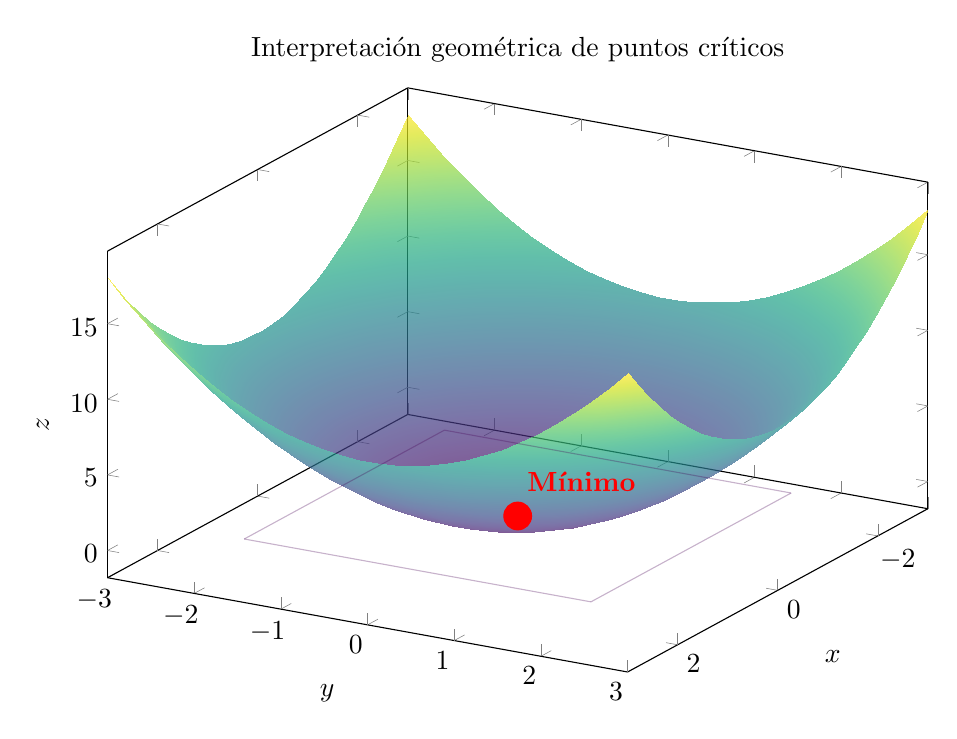
\begin{tikzpicture}
  \begin{axis}[
      view={120}{30},
      width=12cm, height=9cm,
      xlabel={$x$}, ylabel={$y$}, zlabel={$z$},
      domain=-3:3, y domain=-3:3,
      samples=30, samples y=30,
      colormap/viridis,
      title={Interpretación geométrica de puntos críticos}
  ]
    % Superficie: paraboloide con mínimo en (0,0,0)
    \addplot3[surf,opacity=0.7,shader=interp] {x^2 + y^2};
    
    % Punto crítico (mínimo)
    \addplot3[only marks, mark=*, mark size=5pt, color=red] coordinates {(0,0,0)};
    \node[anchor=south west,text=red] at (axis cs:0,0,1) {\textbf{Mínimo}};
    
    % Plano tangente (horizontal en el mínimo)
    \addplot3[gray!30,mesh,opacity=0.3] coordinates {
      (-2,-2,0) (-2,2,0) (2,2,0) (2,-2,0) (-2,-2,0)
    };
  \end{axis}
\end{tikzpicture}
\caption{Punto crítico en $(0,0,0)$: plano tangente horizontal (mínimo).}
\label{fig:punto_critico_minimo}
\end{figure}

\paragraph{Procedimiento para encontrar puntos críticos.}

\textbf{Paso 1:} Calcular las derivadas parciales $f_x$ y $f_y$

\textbf{Paso 2:} Establecer el sistema de ecuaciones:
\begin{align*}
f_x(x,y) &= 0 \\
f_y(x,y) &= 0
\end{align*}

\textbf{Paso 3:} Resolver el sistema para obtener los puntos $(x_0, y_0)$

\textbf{Paso 4:} Verificar cada solución (algunos sistemas pueden no tener solución o tener infinitas)

\begin{EjercicioBox}[Ejemplo 1: Función polinomial simple]
Encontrar los puntos críticos de $f(x,y) = x^2 + y^2 - 4x + 6y + 5$.

\textbf{Solución:}

\textbf{Paso 1:} Calcular las derivadas parciales
\begin{align*}
\frac{\partial f}{\partial x} &= 2x - 4 \\
\frac{\partial f}{\partial y} &= 2y + 6
\end{align*}

\textbf{Paso 2:} Establecer el sistema
\begin{align*}
2x - 4 &= 0 \\
2y + 6 &= 0
\end{align*}

\textbf{Paso 3:} Resolver
\begin{align*}
x &= 2 \\
y &= -3
\end{align*}

\textbf{Resultado:} El único punto crítico es $\boxed{(2, -3)}$.

\textbf{Verificación:} $f(2,-3) = 4 + 9 - 8 - 18 + 5 = -8$. Podemos reescribir la función completando cuadrados:
\[
f(x,y) = (x-2)^2 + (y+3)^2 - 8
\]

Esto confirma que $(2, -3)$ es un mínimo absoluto con valor $-8$.
\end{EjercicioBox}

\begin{EjercicioBox}[Ejemplo 2: Función con términos mixtos]
Encontrar los puntos críticos de $f(x,y) = x^3 + y^3 - 3xy$.

\textbf{Solución:}

\textbf{Paso 1:} Derivadas parciales
\begin{align*}
\frac{\partial f}{\partial x} &= 3x^2 - 3y \\
\frac{\partial f}{\partial y} &= 3y^2 - 3x
\end{align*}

\textbf{Paso 2:} Sistema de ecuaciones
\begin{align*}
3x^2 - 3y &= 0 \implies y = x^2 \tag{1} \\
3y^2 - 3x &= 0 \implies x = y^2 \tag{2}
\end{align*}

\textbf{Paso 3:} Resolver sustituyendo (1) en (2)
\begin{align*}
x &= (x^2)^2 \\
x &= x^4 \\
x^4 - x &= 0 \\
x(x^3 - 1) &= 0
\end{align*}

Esto da $x = 0$ o $x = 1$.

Para $x = 0$: $y = 0^2 = 0$ → Punto crítico: $(0, 0)$

Para $x = 1$: $y = 1^2 = 1$ → Punto crítico: $(1, 1)$

\textbf{Resultado:} Los puntos críticos son $\boxed{(0,0) \text{ y } (1,1)}$.

\textbf{Nota:} Para determinar si son máximos, mínimos o puntos de silla, necesitaríamos la prueba de la segunda derivada (que veremos en la siguiente sección).
\end{EjercicioBox}

\begin{EjercicioBox}[Ejemplo 3: Función exponencial]
Encontrar los puntos críticos de $f(x,y) = e^{x+y}(x^2 - 2y^2)$.

\textbf{Solución:}

\textbf{Paso 1:} Calcular las derivadas parciales usando la regla del producto

\begin{align*}
\frac{\partial f}{\partial x} &= e^{x+y}(x^2 - 2y^2) + e^{x+y}(2x) \\
&= e^{x+y}(x^2 + 2x - 2y^2)
\end{align*}

\begin{align*}
\frac{\partial f}{\partial y} &= e^{x+y}(x^2 - 2y^2) + e^{x+y}(-4y) \\
&= e^{x+y}(x^2 - 2y^2 - 4y)
\end{align*}

\textbf{Paso 2:} Establecer el sistema. Como $e^{x+y} \neq 0$ para todo $(x,y)$:
\begin{align*}
x^2 + 2x - 2y^2 &= 0 \tag{1} \\
x^2 - 2y^2 - 4y &= 0 \tag{2}
\end{align*}

\textbf{Paso 3:} Restar (2) de (1)
\begin{align*}
(x^2 + 2x - 2y^2) - (x^2 - 2y^2 - 4y) &= 0 \\
2x + 4y &= 0 \\
x &= -2y \tag{3}
\end{align*}

\textbf{Paso 4:} Sustituir (3) en (2)
\begin{align*}
(-2y)^2 - 2y^2 - 4y &= 0 \\
4y^2 - 2y^2 - 4y &= 0 \\
2y^2 - 4y &= 0 \\
2y(y - 2) &= 0
\end{align*}

Entonces $y = 0$ o $y = 2$.

Para $y = 0$: $x = 0$ → Punto: $(0, 0)$

Para $y = 2$: $x = -4$ → Punto: $(-4, 2)$

\textbf{Resultado:} Los puntos críticos son $\boxed{(0,0) \text{ y } (-4,2)}$.
\end{EjercicioBox}

\begin{EjercicioBox}[Ejemplo 4: Sistema con una única solución (función racional)]
Encontrar los puntos críticos de $f(x,y) = \frac{1}{x^2 + y^2 + 1}$.

\textbf{Solución:}

\textbf{Paso 1:} Derivadas parciales (usando la regla de la cadena)
\begin{align*}
\frac{\partial f}{\partial x} &= \frac{-2x}{(x^2 + y^2 + 1)^2} \\
\frac{\partial f}{\partial y} &= \frac{-2y}{(x^2 + y^2 + 1)^2}
\end{align*}

\textbf{Paso 2:} Sistema de ecuaciones. El denominador nunca es cero, así:
\begin{align*}
-2x &= 0 \implies x = 0 \\
-2y &= 0 \implies y = 0
\end{align*}

\textbf{Resultado:} El único punto crítico es $\boxed{(0, 0)}$ con valor $f(0,0) = 1$ (máximo absoluto).
\end{EjercicioBox}

\begin{EjercicioBox}[Ejemplo 5: Función de tres variables]
Encontrar los puntos críticos de $f(x,y,z) = x^2 + 2y^2 + 3z^2 - 2x + 4y - 6z + 5$.

\textbf{Solución:}

\textbf{Paso 1:} Derivadas parciales
\begin{align*}
\frac{\partial f}{\partial x} &= 2x - 2 \\
\frac{\partial f}{\partial y} &= 4y + 4 \\
\frac{\partial f}{\partial z} &= 6z - 6
\end{align*}

\textbf{Paso 2:} Sistema
\begin{align*}
2x - 2 &= 0 \implies x = 1 \\
4y + 4 &= 0 \implies y = -1 \\
6z - 6 &= 0 \implies z = 1
\end{align*}

\textbf{Resultado:} El único punto crítico es $\boxed{(1, -1, 1)}$ con valor $f(1,-1,1) = 1 - 2 + 3 - 2 - 4 - 6 + 5 = -5$.

Completando cuadrados podemos verificar:
\[
f(x,y,z) = (x-1)^2 + 2(y+1)^2 + 3(z-1)^2 - 5
\]

El punto es un mínimo absoluto.
\end{EjercicioBox}

\paragraph{Clasificación de puntos críticos.}

No todos los puntos críticos son máximos o mínimos. Existen tres tipos:

\begin{InfoBox}
\Meta{Tipos de puntos críticos}{}

\textbf{1. Máximo local:} La función alcanza su valor más grande en una vecindad del punto.

\textbf{2. Mínimo local:} La función alcanza su valor más pequeño en una vecindad del punto.

\textbf{3. Punto de silla:} El punto es máximo en algunas direcciones y mínimo en otras.

\Meta{Nota importante}{Para determinar el tipo de punto crítico, se usa el \textbf{test de la segunda derivada parcial} (matriz Hessiana), que estudiaremos en la siguiente subsección.}
\end{InfoBox}

\paragraph{Condiciones necesarias vs. suficientes.}

\begin{InfoBox}
\Meta{Teorema (Condición necesaria)}{Si $f(x,y)$ tiene un extremo local en $(x_0, y_0)$ y las derivadas parciales existen en ese punto, entonces:}
\[
\frac{\partial f}{\partial x}(x_0, y_0) = 0 \quad \text{y} \quad \frac{\partial f}{\partial y}(x_0, y_0) = 0
\]

\Meta{Importante}{Esta es una condición \textbf{necesaria} pero \textbf{NO suficiente}. Un punto crítico puede no ser extremo (puede ser punto de silla).}

\Meta{Observación}{La condición se vuelve suficiente si se combina con la prueba de la segunda derivada (veremos próximamente).}
\end{InfoBox}

\paragraph{Puntos críticos en contextos aplicados.}

\begin{TemaBox}[Aplicaciones prácticas de puntos críticos]

\textbf{1. Economía y negocios:}
\begin{itemize}
  \item \textbf{Optimización de utilidades:} Encontrar producción $(x, y)$ que maximice ganancia $P(x,y) = R(x,y) - C(x,y)$
  \item \textbf{Análisis de precios:} Determinar precios óptimos para dos productos minimizando costos
\end{itemize}

\textbf{2. Física e ingeniería:}
\begin{itemize}
  \item \textbf{Principio de energía mínima:} Los sistemas tienden a estados de energía mínima
  \item \textbf{Equilibrio:} Puntos críticos de la energía potencial son puntos de equilibrio
\end{itemize}

\textbf{3. Machine Learning:}
\begin{itemize}
  \item \textbf{Entrenamiento de redes neuronales:} Minimizar función de pérdida
  \item \textbf{Regresión:} Encontrar parámetros que ajusten mejor los datos
\end{itemize}

\textbf{4. Estadística:}
\begin{itemize}
  \item \textbf{Estimación MLE:} Maximizar función de verosimilitud
  \item \textbf{Análisis de varianza:} Optimizar modelos de regresión multivariable
\end{itemize}

\textbf{5. Control ambiental:}
\begin{itemize}
  \item \textbf{Monitoreo de contaminación:} Localizar fuentes de contaminación en dos/tres dimensiones
  \item \textbf{Modelado de calidad de aire:} Puntos críticos en concentraciones de contaminantes
\end{itemize}

\end{TemaBox}

\begin{EjercicioBox}[Aplicación 1: Optimización de producción]
Una empresa produce dos tipos de productos cuya ganancia está dada por:
\[
P(x,y) = 100x + 120y - x^2 - 2y^2 - xy + 1000
\]

donde $x$ e $y$ son unidades producidas (en cientos) de cada producto.

Encontrar los niveles de producción que maximizan la ganancia.

\textbf{Solución:}

\textbf{Paso 1:} Derivadas parciales
\begin{align*}
\frac{\partial P}{\partial x} &= 100 - 2x - y \\
\frac{\partial P}{\partial y} &= 120 - 4y - x
\end{align*}

\textbf{Paso 2:} Establecer el sistema para puntos críticos
\begin{align*}
100 - 2x - y &= 0 \implies 2x + y = 100 \tag{1} \\
120 - 4y - x &= 0 \implies x + 4y = 120 \tag{2}
\end{align*}

\textbf{Paso 3:} Resolver. De (1): $y = 100 - 2x$

Sustituir en (2):
\begin{align*}
x + 4(100 - 2x) &= 120 \\
x + 400 - 8x &= 120 \\
-7x &= -280 \\
x &= 40
\end{align*}

De (1): $y = 100 - 80 = 20$

\textbf{Resultado:} El punto crítico es $(40, 20)$ (4000 unidades del primer producto, 2000 del segundo).

\textbf{Ganancia máxima:}
\[
P(40, 20) = 100(40) + 120(20) - 40^2 - 2(20)^2 - (40)(20) + 1000
\]
\[
= 4000 + 2400 - 1600 - 800 - 800 + 1000 = 4200
\]

La ganancia máxima es $\boxed{4200}$ unidades monetarias.
\end{EjercicioBox}

\begin{EjercicioBox}[Aplicación 2: Diseño de envase con volumen mínimo]
Se desea diseñar una caja rectangular sin tapa, con volumen $V = 1000$ cm$^3$. El costo de material es:
\[
C(x,y) = 2xy + 10x \cdot h + 10y \cdot h
\]

donde $x$ e $y$ son las dimensiones de la base (en cm) y $h = \frac{1000}{xy}$ es la altura (en cm).

Encontrar las dimensiones que minimizan el costo.

\textbf{Solución:}

Sustituyendo $h = \frac{1000}{xy}$:

\begin{align*}
C(x,y) &= 2xy + 10x \cdot \frac{1000}{xy} + 10y \cdot \frac{1000}{xy} \\
&= 2xy + \frac{10000}{y} + \frac{10000}{x}
\end{align*}

\textbf{Derivadas parciales:}
\begin{align*}
\frac{\partial C}{\partial x} &= 2y - \frac{10000}{x^2} \\
\frac{\partial C}{\partial y} &= 2x - \frac{10000}{y^2}
\end{align*}

\textbf{Sistema de ecuaciones:}
\begin{align*}
2y - \frac{10000}{x^2} &= 0 \implies y = \frac{5000}{x^2} \tag{1} \\
2x - \frac{10000}{y^2} &= 0 \implies x = \frac{5000}{y^2} \tag{2}
\end{align*}

\textbf{Resolver:} De (1) en (2):
\begin{align*}
x &= \frac{5000}{(5000/x^2)^2} = \frac{5000 \cdot x^4}{25000000} = \frac{x^4}{5000}
\end{align*}

Simplificando: $5000 = x^3$, entonces $x = \sqrt[3]{5000} \approx 17.1$ cm

De (1): $y = \frac{5000}{(17.1)^2} \approx 17.1$ cm

Por simetría del sistema: $x = y = \sqrt[3]{5000}$ cm

\textbf{Altura:} $h = \frac{1000}{xy} = \frac{1000}{(\sqrt[3]{5000})^2} = \sqrt[3]{250} \approx 6.3$ cm

\textbf{Resultado:} Las dimensiones óptimas son aproximadamente $\boxed{17.1 \times 17.1 \times 6.3 \text{ cm}}$ (base cuadrada).
\end{EjercicioBox}

\paragraph{Dificultades comunes al encontrar puntos críticos.}

\begin{itemize}
  \item \textbf{Sistemas no lineales complejos:} Algunos sistemas no tienen soluciones analíticas. En estos casos, se usan métodos numéricos (Newton-Raphson, etc.)
  
  \item \textbf{Soluciones infinitas:} A veces el sistema tiene infinitas soluciones (toda una curva o región). Esto indica que la función es constante en esa región.
  
  \item \textbf{Puntos donde las derivadas no existen:} Estos también son candidatos a extremos. Por ejemplo, $f(x,y) = |x| + |y|$ tiene un mínimo en $(0,0)$ aunque las derivadas no existen ahí.
  
  \item \textbf{Confundir puntos críticos con extremos:} Recordar que encontrar puntos críticos es solo el primer paso; hay que clasificarlos usando la prueba de la segunda derivada.
\end{itemize}

\paragraph{Ejercicios propuestos.}

Encontrar todos los puntos críticos de las siguientes funciones:

\begin{enumerate}
  \item $f(x,y) = x^2 + 2y^2 - 4x + 8y + 3$
  
  \item $f(x,y) = x^3 + y^3 - 12xy$
  
  \item $f(x,y) = xe^{-x^2-y^2}$
  
  \item $f(x,y) = \frac{x}{y^2 + 1}$ (Sugerencia: después de derivar, note que el numerador es más importante)
  
  \item $f(x,y,z) = x^2 + y^2 + z^2 - xy - xz - yz$
  
  \item Una caja rectangular tiene volumen fijo de 500 m$^3$. El costo de construcción es: suelo $\$5$/m$^2$, paredes $\$3$/m$^2$, techo $\$2$/m$^2$. Si las dimensiones de la base son $x$ e $y$, y la altura es $z$, encuentre las dimensiones que minimizan el costo total.
  
  \item Para la función $f(x,y) = x^4 + y^4 - 4xy$, encuentre los puntos críticos e intente clasificarlos observando el gráfico (usando software si es necesario).
  
  \item Demostrar que la función $f(x,y) = x^2 - y^2$ tiene un punto crítico en $(0,0)$ que es un punto de silla.
\end{enumerate}

\subsubsection{Máximos}

\begin{TemaBox}[Máximos de funciones multivariables: Teoría y aplicaciones]
Los máximos de funciones de varias variables representan los puntos donde la función alcanza sus valores más grandes en una región dada. El análisis de máximos es crucial en optimización, economía, diseño de ingeniería y problemas de control. A diferencia de una variable, una función multivariable puede tener múltiples máximos locales, y distinguir entre máximos locales y globales requiere técnicas especializadas.
\end{TemaBox}

\paragraph{Introducción.}

Un máximo de una función multivariable $f(x,y)$ es un punto donde la función alcanza un valor mayor o igual al de todos los puntos en una vecindad. En el contexto de optimización:

\begin{itemize}
  \item \textbf{Máximo local:} $f(x_0, y_0) \geq f(x,y)$ para todo $(x,y)$ en una vecindad de $(x_0, y_0)$
  \item \textbf{Máximo global:} $f(x_0, y_0) \geq f(x,y)$ para todos los puntos en el dominio
  \item \textbf{Máximo absoluto:} Sinónimo de máximo global
  \item \textbf{Máximo relativo:} Sinónimo de máximo local
\end{itemize}

\paragraph{Definición formal de máximos.}

\begin{InfoBox}
\Meta{Definición (Máximo local)}{Sea $f(x,y)$ una función definida en una región $D$ del plano. Un punto $(x_0, y_0) \in D$ es un \textbf{máximo local} de $f$ si existe un disco abierto $B$ centrado en $(x_0, y_0)$ tal que:}
\[
f(x_0, y_0) \geq f(x,y) \quad \text{para todo } (x,y) \in B \cap D
\]

\Meta{Definición (Máximo global)}{Un punto $(x_0, y_0)$ es un \textbf{máximo global} (o absoluto) si:}
\[
f(x_0, y_0) \geq f(x,y) \quad \text{para todo } (x,y) \in D
\]

\Meta{Valor del máximo}{El \textbf{valor máximo} es el número $f(x_0, y_0)$, mientras que $(x_0, y_0)$ es el \textbf{punto donde se alcanza} el máximo.}
\end{InfoBox}

\paragraph{Caracterización de máximos mediante la prueba de la segunda derivada.}

Para clasificar un punto crítico como máximo, usamos la \textbf{matriz Hessiana}:

\begin{InfoBox}
\Meta{Matriz Hessiana}{Para una función $f(x,y)$ de clase $C^2$, la matriz Hessiana en un punto es:}
\[
H(x,y) = \begin{pmatrix}
f_{xx}(x,y) & f_{xy}(x,y) \\
f_{yx}(x,y) & f_{yy}(x,y)
\end{pmatrix}
\]

donde $f_{xx} = \frac{\partial^2 f}{\partial x^2}$, $f_{xy} = \frac{\partial^2 f}{\partial x \partial y}$, etc.

\Meta{Determinante Hessiano}{Se define:}
\[
D = \det(H) = f_{xx} \cdot f_{yy} - (f_{xy})^2
\]

\Meta{Prueba de la segunda derivada (2D)}{Sea $(x_0, y_0)$ un punto crítico de $f$ donde $f_x = f_y = 0$:}

\begin{itemize}
  \item \textbf{Si $D > 0$ y $f_{xx} < 0$:} $(x_0, y_0)$ es un \textbf{máximo local}
  \item \textbf{Si $D > 0$ y $f_{xx} > 0$:} $(x_0, y_0)$ es un mínimo local
  \item \textbf{Si $D < 0$:} $(x_0, y_0)$ es un \textbf{punto de silla}
  \item \textbf{Si $D = 0$:} El test es \textbf{no conclusivo}
\end{itemize}
\end{InfoBox}

\paragraph{Procedimiento sistemático para encontrar máximos.}

\textbf{Paso 1:} Encontrar todos los puntos críticos resolviendo $\nabla f = \mathbf{0}$

\textbf{Paso 2:} Para cada punto crítico $(x_0, y_0)$:
\begin{itemize}
  \item Calcular las segundas derivadas parciales: $f_{xx}$, $f_{yy}$, $f_{xy}$
  \item Evaluar estas derivadas en el punto crítico
  \item Calcular $D = f_{xx} \cdot f_{yy} - (f_{xy})^2$
\end{itemize}

\textbf{Paso 3:} Clasificar usando la prueba de la segunda derivada

\textbf{Paso 4:} Para máximos globales, comparar valores en todos los máximos locales y en la frontera (si existe)

\begin{EjercicioBox}[Ejemplo 1: Paraboloide - máximo único]
Encontrar y clasificar los puntos críticos de $f(x,y) = -x^2 - y^2 + 4x + 6y - 5$.

\textbf{Solución:}

\textbf{Paso 1:} Encontrar puntos críticos
\begin{align*}
\frac{\partial f}{\partial x} &= -2x + 4 = 0 \implies x = 2 \\
\frac{\partial f}{\partial y} &= -2y + 6 = 0 \implies y = 3
\end{align*}

Punto crítico: $(2, 3)$

\textbf{Paso 2:} Calcular segundas derivadas
\begin{align*}
f_{xx} &= -2 \\
f_{yy} &= -2 \\
f_{xy} &= 0
\end{align*}

\textbf{Paso 3:} Aplicar prueba de segunda derivada
\begin{align*}
D &= f_{xx} \cdot f_{yy} - (f_{xy})^2 \\
&= (-2)(-2) - 0^2 \\
&= 4 > 0
\end{align*}

Como $D = 4 > 0$ y $f_{xx} = -2 < 0$:

\textbf{Resultado:} $(2, 3)$ es un \textbf{máximo local}.

\textbf{Valor máximo:} $f(2,3) = -4 - 9 + 8 + 18 - 5 = 8$

\textbf{Verificación:} Completando cuadrados:
\[
f(x,y) = -(x-2)^2 - (y-3)^2 + 8
\]

Esto confirma que $(2,3)$ es máximo absoluto con valor 8.
\end{EjercicioBox}

\begin{EjercicioBox}[Ejemplo 2: Función con punto de silla]
Analizar $f(x,y) = x^3 - 3xy + y^3$.

\textbf{Solución:}

\textbf{Paso 1:} Puntos críticos
\begin{align*}
\frac{\partial f}{\partial x} &= 3x^2 - 3y = 0 \implies y = x^2 \\
\frac{\partial f}{\partial y} &= -3x + 3y^2 = 0 \implies y^2 = x
\end{align*}

De $y = x^2$ y $y^2 = x$:
\begin{align*}
(x^2)^2 &= x \\
x^4 &= x \\
x(x^3 - 1) &= 0
\end{align*}

Entonces $x = 0$ o $x = 1$.

- Para $x = 0$: $y = 0$ → Punto: $(0, 0)$
- Para $x = 1$: $y = 1$ → Punto: $(1, 1)$

\textbf{Paso 2:} Segundas derivadas
\begin{align*}
f_{xx} &= 6x \\
f_{yy} &= 6y \\
f_{xy} &= -3
\end{align*}

\textbf{Paso 3:} Clasificar en $(0, 0)$
\begin{align*}
f_{xx}(0,0) &= 0 \\
f_{yy}(0,0) &= 0 \\
f_{xy}(0,0) &= -3 \\
D &= 0 \cdot 0 - (-3)^2 = -9 < 0
\end{align*}

Como $D < 0$: $(0,0)$ es un \textbf{punto de silla}.

\textbf{Paso 4:} Clasificar en $(1, 1)$
\begin{align*}
f_{xx}(1,1) &= 6 \\
f_{yy}(1,1) &= 6 \\
f_{xy}(1,1) &= -3 \\
D &= 6 \cdot 6 - (-3)^2 = 36 - 9 = 27 > 0
\end{align*}

Como $D = 27 > 0$ y $f_{xx} = 6 > 0$: $(1,1)$ es un \textbf{mínimo local}

\textbf{Resultado:} La función tiene un punto de silla en $(0,0)$ y mínimo local en $(1,1)$. No tiene máximos locales.
\end{EjercicioBox}

\begin{EjercicioBox}[Ejemplo 3: Función racional con máximo]
Analizar $f(x,y) = \frac{1}{1 + x^2 + y^2}$.

\textbf{Solución:}

\textbf{Paso 1:} Puntos críticos
\begin{align*}
\frac{\partial f}{\partial x} &= \frac{-2x}{(1+x^2+y^2)^2} = 0 \implies x = 0 \\
\frac{\partial f}{\partial y} &= \frac{-2y}{(1+x^2+y^2)^2} = 0 \implies y = 0
\end{align*}

Punto crítico: $(0, 0)$

\textbf{Paso 2:} Segundas derivadas (en el origen)
\[
\frac{\partial^2 f}{\partial x^2} = \frac{\partial}{\partial x}\left[\frac{-2x}{(1+x^2+y^2)^2}\right]
\]

Aplicando regla del cociente:
\[
f_{xx} = \frac{-2(1+x^2+y^2)^2 - (-2x) \cdot 2(1+x^2+y^2) \cdot 2x}{(1+x^2+y^2)^4}
\]

En $(0,0)$:
\[
f_{xx}(0,0) = \frac{-2}{1} = -2
\]

Por simetría: $f_{yy}(0,0) = -2$

Para $f_{xy}$: El término con $xy$ en numerador da $f_{xy}(0,0) = 0$

\textbf{Paso 3:} Prueba de segunda derivada
\begin{align*}
D &= f_{xx} \cdot f_{yy} - (f_{xy})^2 \\
&= (-2)(-2) - 0 = 4 > 0
\end{align*}

Como $D > 0$ y $f_{xx} = -2 < 0$: $(0,0)$ es \textbf{máximo local}

\textbf{Valor máximo:} $f(0,0) = 1$

\textbf{Interpretación:} Es máximo \textbf{global absoluto} porque la función $\to 0$ cuando $(x,y) \to \infty$
\end{EjercicioBox}

\begin{EjercicioBox}[Ejemplo 4: Paraboloide hiperbólico (silla)]
Analizar $f(x,y) = x^2 - 2xy + y^2 + 2x - 2y$.

\textbf{Solución:}

\textbf{Paso 1:} Puntos críticos
\begin{align*}
\frac{\partial f}{\partial x} &= 2x - 2y + 2 = 0 \implies x - y = -1 \\
\frac{\partial f}{\partial y} &= -2x + 2y - 2 = 0 \implies -x + y = 1
\end{align*}

Ambas ecuaciones son idénticas: $y = x + 1$

En realidad, tenemos un sistema compatible indeterminado. Toda la línea $y = x + 1$ son puntos críticos.

Esto indica que la función puede reescribirse. Completando:
\[
f(x,y) = (x-y)^2 + 2(x-y)
\]

Sea $u = x - y$:
\[
f = u^2 + 2u = (u+1)^2 - 1 = (x-y+1)^2 - 1
\]

\textbf{Resultado:} 
- Mínimo de $-1$ cuando $x - y = -1$ (toda la línea $y = x + 1$)
- La función no tiene máximos locales (es ilimitada superiormente)
- El conjunto de mínimos forma una línea, no un punto aislado
\end{EjercicioBox}

\begin{EjercicioBox}[Ejemplo 5: Función con máximos múltiples]
Analizar $f(x,y) = \sin(x) \sin(y)$ en el dominio $[0, 2\pi] \times [0, 2\pi]$.

\textbf{Solución:}

\textbf{Paso 1:} Puntos críticos
\begin{align*}
\frac{\partial f}{\partial x} &= \cos(x) \sin(y) = 0 \\
\frac{\partial f}{\partial y} &= \sin(x) \cos(y) = 0
\end{align*}

De la primera: $\cos(x) = 0$ o $\sin(y) = 0$  
De la segunda: $\sin(x) = 0$ o $\cos(y) = 0$

Si $\sin(x) = 0$: $x \in \{0, \pi, 2\pi\}$  
Si $\cos(x) = 0$: $x \in \{\pi/2, 3\pi/2\}$

Similarmente para $y$.

Los puntos críticos en el interior son:
- $(\pi/2, \pi/2)$: $f = 1 \cdot 1 = 1$ ← **MÁXIMO**
- $(\pi/2, 3\pi/2)$: $f = 1 \cdot (-1) = -1$ ← Mínimo
- $(3\pi/2, \pi/2)$: $f = (-1) \cdot 1 = -1$ ← Mínimo
- $(3\pi/2, 3\pi/2)$: $f = (-1)(-1) = 1$ ← **MÁXIMO**

En la frontera: $f = 0$ (porque siempre hay un $\sin$ nulo)

\textbf{Resultado:} 
- Hay dos máximos locales (y globales) con valor 1 en $(\pi/2, \pi/2)$ y $(3\pi/2, 3\pi/2)$
- Hay dos mínimos locales con valor $-1$ en $(\pi/2, 3\pi/2)$ y $(3\pi/2, \pi/2)$
\end{EjercicioBox}

\paragraph{Teorema de Weierstrass y máximos globales.}

\begin{InfoBox}
\Meta{Teorema de Weierstrass}{Si $f(x,y)$ es continua en un conjunto compacto $D$ (cerrado y acotado), entonces $f$ alcanza su máximo y mínimo absolutos en $D$.}

\Meta{Cómo encontrar máximos globales en un compacto}{}
\begin{enumerate}
  \item Encontrar todos los máximos locales en el interior (puntos críticos)
  \item Encontrar todos los máximos en la frontera (usando multiplicadores de Lagrange o parametrización)
  \item Comparar todos los valores encontrados
  \item El mayor valor es el máximo global
\end{enumerate}

\Meta{Corolario}{En un dominio abierto no acotado, puede no existir máximo global (la función puede ser ilimitada).}
\end{InfoBox}

\paragraph{Aplicaciones prácticas de máximos.}

\begin{TemaBox}[Aplicaciones de máximos en contextos reales]

\textbf{1. Economía y negocios:}
\begin{itemize}
  \item Maximizar ingresos: $R(p_1, p_2) = p_1 q_1(p_1, p_2) + p_2 q_2(p_1, p_2)$
  \item Maximizar utilidad: $U(x,y) = f(x,y) - C(x,y)$
  \item Optimización de portafolio: máxima rentabilidad con riesgo dado
\end{itemize}

\textbf{2. Ingeniería y diseño:}
\begin{itemize}
  \item Maximizar resistencia estructural
  \item Maximizar eficiencia energética
  \item Maximizar producción con recursos limitados
\end{itemize}

\textbf{3. Biología y medicina:}
\begin{itemize}
  \item Maximizar crecimiento de población
  \item Maximizar efectividad de tratamientos
  \item Optimizar dosis de medicamentos
\end{itemize}

\textbf{4. Machine Learning:}
\begin{itemize}
  \item Maximizar precisión del modelo
  \item Maximizar área bajo la curva ROC
  \item Maximizar función de verosimilitud
\end{itemize}

\textbf{5. Física:}
\begin{itemize}
  \item Principio de máxima entropía
  \item Trayectorias de máxima probabilidad
  \item Configuración de máxima estabilidad
\end{itemize}

\end{TemaBox}

\begin{EjercicioBox}[Aplicación 1: Maximización de ingresos empresariales]
Una empresa vende dos productos. Los ingresos están dados por:
\[
R(x,y) = 100x + 120y - x^2 - 2xy - \frac{3y^2}{2} - 50
\]

donde $x$ e $y$ son las cantidades vendidas.

Encontrar el nivel de ventas que maximiza los ingresos.

\textbf{Solución:}

\textbf{Paso 1:} Encontrar puntos críticos
\begin{align*}
\frac{\partial R}{\partial x} &= 100 - 2x - 2y = 0 \\
\frac{\partial R}{\partial y} &= 120 - 2x - 3y = 0
\end{align*}

De la primera: $2x + 2y = 100 \implies x + y = 50$

De la segunda: $2x + 3y = 120$

Restando: $y = 20$, entonces $x = 30$

Punto crítico: $(30, 20)$

\textbf{Paso 2:} Segundas derivadas
\begin{align*}
R_{xx} &= -2 \\
R_{yy} &= -3 \\
R_{xy} &= -2
\end{align*}

\textbf{Paso 3:} Prueba de segunda derivada
\begin{align*}
D &= R_{xx} \cdot R_{yy} - (R_{xy})^2 \\
&= (-2)(-3) - (-2)^2 \\
&= 6 - 4 = 2 > 0
\end{align*}

Como $D > 0$ y $R_{xx} = -2 < 0$: $(30, 20)$ es **máximo local**

\textbf{Ingresos máximos:}
\begin{align*}
R(30, 20) &= 100(30) + 120(20) - 900 - 2(30)(20) - \frac{3(400)}{2} - 50 \\
&= 3000 + 2400 - 900 - 1200 - 600 - 50 \\
&= 2650 \text{ unidades monetarias}
\end{align*}

\textbf{Interpretación:} Vender 30 unidades del producto 1 y 20 del producto 2 maximiza los ingresos en 2650 unidades.
\end{EjercicioBox}

\begin{EjercicioBox}[Aplicación 2: Diseño óptimo de recipiente]
Se desea diseñar un tanque rectangular abierto (sin tapa) de volumen $V = 32$ m³ minimizando la superficie de material (pero maximizando la eficiencia del espacio por unidad de material).

Si las dimensiones de la base son $x$ e $y$, y la altura es $h = \frac{32}{xy}$, la superficie es:
\[
S(x,y) = xy + 2xh + 2yh = xy + \frac{64}{y} + \frac{64}{x}
\]

Encontrar las dimensiones que minimizan la superficie (o equivalentemente, que maxinimizan volumen/área).

\textbf{Solución:}

\textbf{Paso 1:} Puntos críticos
\begin{align*}
\frac{\partial S}{\partial x} &= y - \frac{64}{x^2} = 0 \implies x^2 y = 64 \\
\frac{\partial S}{\partial y} &= x - \frac{64}{y^2} = 0 \implies xy^2 = 64
\end{align*}

De las dos ecuaciones:
\[
\frac{x^2 y}{xy^2} = \frac{x}{y} = 1 \implies x = y
\]

Sustituyendo en la primera: $x^3 = 64 \implies x = 4$

Punto crítico: $(4, 4)$ con altura $h = \frac{32}{16} = 2$

\textbf{Paso 2:} Segundas derivadas
\begin{align*}
S_{xx} &= \frac{128}{x^3} \\
S_{yy} &= \frac{128}{y^3} \\
S_{xy} &= 1
\end{align*}

En $(4,4)$:
\begin{align*}
S_{xx}(4,4) &= \frac{128}{64} = 2 \\
S_{yy}(4,4) &= 2 \\
S_{xy}(4,4) &= 1
\end{align*}

\textbf{Paso 3:} Prueba de segunda derivada
\begin{align*}
D &= 2 \cdot 2 - 1^2 = 4 - 1 = 3 > 0
\end{align*}

Como $D > 0$ y $S_{xx} = 2 > 0$: $(4, 4)$ es un **mínimo** (no máximo)

\textbf{Resultado:} 
- Dimensiones óptimas: base cuadrada de 4 m × 4 m
- Altura: 2 m
- Superficie mínima: $S(4,4) = 16 + 16 + 16 = 48$ m²

(Nota: En este problema buscábamos minimizar superficie, lo que da contexto al máximo de eficiencia volumen/área)
\end{EjercicioBox}

\paragraph{Comparación: máximos locales vs. globales.}

\begin{itemize}
  \item \textbf{Máximo local:} Mayor que en vecinos inmediatos. Puede haber múltiples en un mismo dominio.
  
  \item \textbf{Máximo global:} Mayor en todo el dominio. Si existe, puede haber uno o varios.
  
  \item \textbf{En dominios abiertos:} Pueden no existir máximos globales (función ilimitada).
  
  \item \textbf{En dominios compactos:} Siempre existen máximos globales (Weierstrass).
  
  \item \textbf{Máximo aislado:} Un único máximo en cierta región.
  
  \item \textbf{Máximos degenerados:} Cuando $D = 0$, la clasificación requiere análisis más profundo.
\end{itemize}

\paragraph{Dificultades al encontrar máximos.}

\begin{itemize}
  \item \textbf{Frontera compleja:} La optimización en la frontera puede ser más difícil que en el interior.
  
  \item \textbf{Máximos no aislados:} El máximo puede darse en una curva o región, no en un punto.
  
  \item \textbf{Singularidades:} Puntos donde las derivadas no existen pueden ser máximos (e.g., $f(x,y) = -|x| - |y|$ tiene máximo en el origen).
  
  \item \textbf{Funciones patológicas:} Algunas funciones continuas no tienen máximos globales en dominios no compactos.
  
  \item \textbf{Dimensión superior:} En 3 o más variables, el Hessiano es una matriz de orden mayor (requiere autovalores).
\end{itemize}

\paragraph{Extensión a funciones de tres variables.}

Para $f(x,y,z)$, la matriz Hessiana es $3 \times 3$:
\[
H = \begin{pmatrix}
f_{xx} & f_{xy} & f_{xz} \\
f_{xy} & f_{yy} & f_{yz} \\
f_{xz} & f_{yz} & f_{zz}
\end{pmatrix}
\]

Un punto crítico es máximo si todos los \textbf{menores principales líderes} negativos forman patrón:
\begin{itemize}
  \item $H_1 = f_{xx} < 0$ (1er menor)
  \item $H_2 = \det\begin{pmatrix} f_{xx} & f_{xy} \\ f_{xy} & f_{yy} \end{pmatrix} > 0$ (2do menor)
  \item $H_3 = \det(H) < 0$ (determinante total)
\end{itemize}

Es decir: \textbf{signos alternados comenzando con negativo}.

\paragraph{Ejercicios propuestos.}

Para cada función, encontrar todos los puntos críticos, clasificarlos y determinar máximos:

\begin{enumerate}
  \item $f(x,y) = 4x + 6y - x^2 - y^2 - 3$
  
  \item $f(x,y) = x^2 - 4xy + 4y^2 + 2x - 4y + 1$
  
  \item $f(x,y) = e^{-(x^2+y^2)}$ (Sugerencia: exponencial es monotónica)
  
  \item $f(x,y) = xy(4-x-y)$ en el dominio $x > 0, y > 0$ (Aplicación de maximizar área)
  
  \item $f(x,y,z) = 4x + 6y + 5z - x^2 - y^2 - z^2$ (3 variables)
  
  \item En un mercado con dos productos complementarios, la ganancia es $\Pi(x,y) = xy - x^2 - y^2 + 10x + 10y - 50$. Encontrar cantidades que maximizan ganancia.
  
  \item Considere $f(x,y) = x^3 + y^3 - 3xy + 5$ y determine si los puntos críticos son máximos, mínimos o puntos de silla.
  
  \item Para $f(x,y) = \sin(x) + \sin(y) + \sin(x+y)$ en $[0, \pi] \times [0, \pi]$, encontrar todos los máximos locales y el máximo global.
\end{enumerate}

\subsubsection{Mínimos}

\begin{TemaBox}[Mínimos de funciones multivariables: Localización y caracterización]
Los mínimos de funciones de varias variables representan los puntos donde la función alcanza sus valores más pequeños en una región dada. A diferencia de los máximos, los mínimos son especialmente importantes en aplicaciones de optimización: minimización de costos, energía, riesgo, o error. El análisis de mínimos es fundamental en ingeniería, economía, estadística y machine learning.
\end{TemaBox}

\paragraph{Introducción.}
En numerosas situaciones prácticas, necesitamos minimizar funciones: reducir costos de producción, minimizar el consumo de energía, disminuir errores en predicciones, o encontrar configuraciones óptimas de sistemas. La caracterización matemática de mínimos en varias variables proporciona herramientas sistemáticas para estos problemas.

\begin{InfoBox}
\textbf{Definiciones fundamentales:}

\Meta{Mínimo Local}{Un punto $(a, b) \in D$ es un \textit{mínimo local} de $f$ si existe una vecindad abierta de $(a, b)$ tal que $f(x, y) \geq f(a, b)$ para todos los puntos $(x, y)$ en esa vecindad. En otras palabras, el valor de la función en $(a, b)$ es menor o igual que en los puntos cercanos.}

\Meta{Mínimo Absoluto o Global}{Un punto $(a, b) \in D$ es un \textit{mínimo absoluto} o \textit{global} de $f$ si $f(x, y) \geq f(a, b)$ para todos los puntos $(x, y)$ en el dominio $D$. Este es el valor más pequeño que la función alcanza en todo el dominio.}

\Meta{Punto Crítico}{Un punto $(a, b)$ es un punto crítico de $f$ si $f_x(a, b) = 0$ y $f_y(a, b) = 0$ simultáneamente. Los mínimos (locales o globales) deben ocurrir en puntos críticos, en la frontera del dominio, o en puntos donde la función no es diferenciable.}
\end{InfoBox}

\paragraph{Criterio de la segunda derivada para mínimos.}
Para una función $f(x, y)$ diferenciable dos veces, el análisis de la matriz Hessiana determina la naturaleza del punto crítico $(a, b)$.

Sea la matriz Hessiana:
\[
H = \begin{pmatrix} f_{xx} & f_{xy} \\ f_{xy} & f_{yy} \end{pmatrix} \text{ evaluada en } (a, b)
\]

Sea $D = f_{xx}(a, b) \cdot f_{yy}(a, b) - [f_{xy}(a, b)]^2$ (determinante de la Hessiana).

\textbf{Criterio para mínimo local:} Si en el punto crítico $(a, b)$:
\begin{itemize}
    \item $D > 0$ \textbf{Y} $f_{xx}(a, b) > 0$, entonces $(a, b)$ es un \textbf{mínimo local}.
    \item Si además $f_{xx}(a, b) > 0$ en todo el dominio y $(a, b)$ es el único punto crítico en $D$, entonces es un \textbf{mínimo global}.
\end{itemize}

\textbf{Otros casos:}
\begin{itemize}
    \item Si $D > 0$ y $f_{xx}(a, b) < 0$: punto de máximo local.
    \item Si $D < 0$: punto de silla (ni máximo ni mínimo).
    \item Si $D = 0$: el criterio es inconcluyente.
\end{itemize}

\paragraph{Procedimiento sistemático para encontrar mínimos.}
\begin{enumerate}
    \item \textbf{Encontrar puntos críticos:} Resolver el sistema $\nabla f = \mathbf{0}$, es decir, $f_x(x, y) = 0$ y $f_y(x, y) = 0$.
    \item \textbf{Calcular derivadas segundas:} Obtener $f_{xx}$, $f_{yy}$, y $f_{xy}$ en cada punto crítico.
    \item \textbf{Evaluar la Hessiana:} Calcular $D = f_{xx} \cdot f_{yy} - (f_{xy})^2$ y verificar $f_{xx} > 0$.
    \item \textbf{Clasificar:} Determinar si es mínimo local, máximo local, o punto de silla.
    \item \textbf{Comparar valores:} Evaluar $f$ en todos los candidatos y en la frontera para hallar el mínimo global.
\end{enumerate}

\begin{EjercicioBox}[Ejemplo 1: Paraboloide elíptico — mínimo único]
Sea $f(x, y) = (x - 2)^2 + 2(y + 1)^2 + 3$.

\textbf{Solución:}

\textit{Paso 1:} Encontrar puntos críticos:
\[
f_x = 2(x - 2) = 0 \quad \Rightarrow \quad x = 2
\]
\[
f_y = 4(y + 1) = 0 \quad \Rightarrow \quad y = -1
\]
Punto crítico único: $(2, -1)$.

\textit{Paso 2:} Derivadas segundas:
\[
f_{xx} = 2, \quad f_{yy} = 4, \quad f_{xy} = 0
\]

\textit{Paso 3:} Evaluar la Hessiana:
\[
D = 2 \cdot 4 - 0^2 = 8 > 0 \quad \text{y} \quad f_{xx} = 2 > 0
\]

\textit{Paso 4:} Conclusión: $(2, -1)$ es un \textbf{mínimo local}. Como $f(x, y) \to \infty$ cuando $||(x, y)|| \to \infty$, este es el \textbf{mínimo global}.

\textit{Valor mínimo:} $f(2, -1) = 0 + 0 + 3 = \boxed{3}$.
\end{EjercicioBox}

\begin{EjercicioBox}[Ejemplo 2: Función cúbica — múltiples puntos críticos]
Sea $f(x, y) = x^3 + y^3 - 3xy$.

\textbf{Solución:}

\textit{Paso 1:} Encontrar puntos críticos:
\[
f_x = 3x^2 - 3y = 0 \quad \Rightarrow \quad y = x^2
\]
\[
f_y = 3y^2 - 3x = 0 \quad \Rightarrow \quad y^2 = x
\]
Sustituyendo $y = x^2$ en $y^2 = x$:
\[
(x^2)^2 = x \quad \Rightarrow \quad x^4 = x \quad \Rightarrow \quad x(x^3 - 1) = 0
\]
Entonces $x = 0$ o $x = 1$.
\begin{itemize}
    \item Si $x = 0$: $y = 0$, punto crítico $(0, 0)$.
    \item Si $x = 1$: $y = 1$, punto crítico $(1, 1)$.
\end{itemize}

\textit{Paso 2:} Derivadas segundas:
\[
f_{xx} = 6x, \quad f_{yy} = 6y, \quad f_{xy} = -3
\]

\textit{Paso 3:} Evaluar en $(0, 0)$:
\[
f_{xx}(0, 0) = 0, \quad f_{yy}(0, 0) = 0, \quad f_{xy}(0, 0) = -3
\]
\[
D(0, 0) = 0 \cdot 0 - (-3)^2 = -9 < 0 \quad \Rightarrow \quad \textbf{punto de silla}
\]

Evaluar en $(1, 1)$:
\[
f_{xx}(1, 1) = 6 > 0, \quad f_{yy}(1, 1) = 6 > 0, \quad f_{xy}(1, 1) = -3
\]
\[
D(1, 1) = 6 \cdot 6 - (-3)^2 = 36 - 9 = 27 > 0 \quad \text{y} \quad f_{xx} = 6 > 0
\]
\[
\Rightarrow \quad \textbf{mínimo local en } (1, 1)
\]

\textit{Valor:} $f(1, 1) = 1 + 1 - 3(1)(1) = 2 - 3 = -1$.
\end{EjercicioBox}

\begin{EjercicioBox}[Ejemplo 3: Función racional con mínimo absoluto]
Sea $f(x, y) = \frac{1}{x^2 + y^2 + 1}$ en $\mathbb{R}^2$.

\textbf{Solución:}

\textit{Paso 1:} Encontrar puntos críticos:
\[
f_x = \frac{-2x}{(x^2 + y^2 + 1)^2} = 0 \quad \Rightarrow \quad x = 0
\]
\[
f_y = \frac{-2y}{(x^2 + y^2 + 1)^2} = 0 \quad \Rightarrow \quad y = 0
\]
Punto crítico único: $(0, 0)$.

\textit{Paso 2:} Análisis: $f(0, 0) = \frac{1}{1} = 1$. Para cualquier $(x, y) \neq (0, 0)$: $x^2 + y^2 > 0$, luego $x^2 + y^2 + 1 > 1$, entonces $\frac{1}{x^2 + y^2 + 1} < 1$.

\textit{Conclusión:} $(0, 0)$ es el \textbf{mínimo global} con $f_{\min} = \boxed{1}$.

\textit{Nota:} $f(x, y) \to 0$ cuando $||(x, y)|| \to \infty$, pero el infimum es 0 sin alcanzarse.
\end{EjercicioBox}

\begin{EjercicioBox}[Ejemplo 4: Función gaussiana — mínimo en frontera]
Sea $f(x, y) = e^{-(x^2 + y^2)}$ en $\mathbb{R}^2$.

\textbf{Solución:}

\textit{Paso 1:} Encontrar puntos críticos:
\[
f_x = -2x \cdot e^{-(x^2 + y^2)} = 0 \quad \Rightarrow \quad x = 0
\]
\[
f_y = -2y \cdot e^{-(x^2 + y^2)} = 0 \quad \Rightarrow \quad y = 0
\]
Punto crítico único: $(0, 0)$.

\textit{Paso 2:} Análisis de naturaleza:
\[
f_{xx} = -2e^{-(x^2 + y^2)} + 4x^2 e^{-(x^2 + y^2)}
\]
En $(0, 0)$: $f_{xx}(0, 0) = -2 < 0$.

\textit{Conclusión:} $(0, 0)$ es un \textbf{máximo local} con $f(0, 0) = 1$.

\textit{Comportamiento:} Como $f(x, y) \to 0$ cuando $||(x, y)|| \to \infty$, el infimum es $0$, aunque es un \textbf{mínimo en el infinito} no local.
\end{EjercicioBox}

\begin{EjercicioBox}[Ejemplo 5: Función con mínimos aislados y estructurados]
Sea $f(x, y) = x^2 \cos(y) + y^2$ en un dominio acotado.

\textbf{Solución:}

\textit{Paso 1:} Encontrar puntos críticos:
\[
f_x = 2x\cos(y) = 0 \quad \Rightarrow \quad x = 0 \text{ o } \cos(y) = 0
\]
\[
f_y = -x^2\sin(y) + 2y = 0
\]

Si $x = 0$: $f_y = 2y = 0 \Rightarrow y = 0$, punto $(0, 0)$.

Si $\cos(y) = 0$: $y = \pi/2 + n\pi$. Entonces $-x^2 \sin(\pi/2 + n\pi) + 2(\pi/2 + n\pi) = 0$, lo que da múltiples puntos críticos.

\textit{Conclusión:} $(0, 0)$ es un candidato a mínimo con $f(0, 0) = 0$. El análisis completo requiere evaluar la Hessiana en todos los candidatos.
\end{EjercicioBox}

\paragraph{Teorema de Weierstrass para mínimos.}
\textbf{Teorema:} Si $f$ es continua en un conjunto compacto $K$ (cerrado y acotado) de $\mathbb{R}^2$, entonces $f$ alcanza su mínimo en $K$. Es decir, existe un punto $(a, b) \in K$ tal que $f(a, b) \leq f(x, y)$ para todo $(x, y) \in K$.

Este teorema garantiza que la búsqueda de mínimos globales en dominios acotados tiene éxito: los mínimos existen y se encuentran bien en puntos críticos interiores o en la frontera del dominio.

\paragraph{Aplicaciones de minimización en varias variables.}

\begin{TemaBox}[Áreas de aplicación de minimización]
\begin{enumerate}
    \item \textbf{Economía:} Minimización de costos de producción, almacenamiento y distribución.
    \item \textbf{Ingeniería:} Diseño óptimo de estructuras, minimización de peso, estrés y consumo energético.
    \item \textbf{Estadística:} Minimización de error cuadrático medio (MSE) en regresión lineal y no lineal.
    \item \textbf{Machine Learning:} Entrenamiento de redes neuronales minimizando función de pérdida.
    \item \textbf{Física:} Mínima energía potencial en sistemas mecánicos y termodinámicos.
\end{enumerate}
\end{TemaBox}

\begin{EjercicioBox}[Aplicación 1: Minimización de costos de producción]
Una fábrica produce dos tipos de artículos. El costo total de producción es:
\[
C(x, y) = 2x^2 + 3y^2 - 4xy + 100x + 50y + 5000
\]
donde $x$ es la cantidad de artículos tipo A (en cientos) e $y$ es la cantidad de artículos tipo B (en cientos).

\textbf{Objetivo:} Encontrar el nivel de producción que minimiza el costo total.

\textbf{Solución:}

\textit{Paso 1:} Encontrar puntos críticos:
\[
C_x = 4x - 4y + 100 = 0
\]
\[
C_y = 6y - 4x + 50 = 0
\]

De la primera ecuación: $4x - 4y = -100 \Rightarrow x - y = -25 \Rightarrow x = y - 25$.

Sustituyendo en la segunda:
\[
6y - 4(y - 25) + 50 = 0 \Rightarrow 6y - 4y + 100 + 50 = 0 \Rightarrow 2y + 150 = 0 \Rightarrow y = -75
\]

Entonces $x = -75 - 25 = -100$.

\textit{Nota económica:} Los valores negativos indican que el modelo de costos es válido solo para producción positiva. En la práctica, se evaluaría en el límite $x, y \geq 0$.

\textit{Paso 2:} Verificar naturaleza del punto crítico:
\[
C_{xx} = 4 > 0, \quad C_{yy} = 6 > 0, \quad C_{xy} = -4
\]
\[
D = 4 \cdot 6 - (-4)^2 = 24 - 16 = 8 > 0 \quad \text{y} \quad C_{xx} = 4 > 0
\]

\textit{Conclusión:} El punto crítico es un mínimo local (aunque no factible económicamente en este caso específico).

\textit{Interpretación:} En dominios factibles (primero cuadrante), se evaluaría el costo en la frontera para encontrar el mínimo práctico.
\end{EjercicioBox}

\begin{EjercicioBox}[Aplicación 2: Optimización de envase cilíndrico con costo mínimo]
Se desea diseñar un envase cilíndrico de volumen $V = 1000$ cm³ que minimice el costo del material. El costo del fondo y tapa es 2 dólares por cm², mientras que el costo de la pared lateral es 1 dólar por cm².

\textbf{Objetivo:} Encontrar dimensiones óptimas (radio $r$ y altura $h$) que minimizan el costo total.

\textbf{Solución:}

\textit{Restricción:} $\pi r^2 h = 1000 \Rightarrow h = \frac{1000}{\pi r^2}$.

\textit{Función objetivo:}
\[
\text{Costo} = C(r, h) = 2 \cdot 2\pi r^2 + 1 \cdot 2\pi r h = 4\pi r^2 + 2\pi rh
\]

Sustituyendo $h$:
\[
C(r) = 4\pi r^2 + 2\pi r \cdot \frac{1000}{\pi r^2} = 4\pi r^2 + \frac{2000}{r}
\]

\textit{Paso 1:} Encontrar mínimos:
\[
C'(r) = 8\pi r - \frac{2000}{r^2} = 0 \Rightarrow 8\pi r^3 = 2000 \Rightarrow r^3 = \frac{250}{\pi}
\]
\[
r = \sqrt[3]{\frac{250}{\pi}} \approx 4.3 \text{ cm}
\]

\textit{Paso 2:} Verificar es mínimo:
\[
C''(r) = 8\pi + \frac{4000}{r^3} > 0 \quad \text{para todo } r > 0
\]

\textit{Conclusión:} El costo es mínimo en $r \approx 4.3$ cm.

\textit{Altura:} $h = \frac{1000}{\pi (4.3)^2} \approx 17.2$ cm.

\textit{Costo mínimo:} $C \approx 4\pi(4.3)^2 + \frac{2000}{4.3} \approx 231 + 465 \approx \$696$.
\end{EjercicioBox}

\paragraph{Comparación: máximos vs. mínimos.}
\begin{enumerate}
    \item \textbf{Condición de primer orden:} En ambos casos, $\nabla f = \mathbf{0}$.
    \item \textbf{Diferencia en segundo orden:} Para mínimos, se requiere $f_{xx} > 0$ (concavidad hacia arriba); para máximos, $f_{xx} < 0$ (concavidad hacia abajo).
    \item \textbf{Simetría:} Si $(a, b)$ es mínimo de $f$, entonces es máximo de $-f$.
    \item \textbf{Aplicaciones:} Mínimos son más comunes en problemas de optimización real (costos, energía, error); máximos aparecen en ganancia, utilidad y potencial.
\end{enumerate}

\paragraph{Dificultades comunes.}
\begin{itemize}
    \item \textbf{Puntos de silla:} Fácilmente confundidos con extremos; requieren análisis completo de la Hessiana.
    \item \textbf{Dominios abiertos:} En dominios abiertos no compactos, el mínimo global puede no existir.
    \item \textbf{Múltiples mínimos:} Funciones no convexas pueden tener varios mínimos locales; encontrar el global requiere métodos de optimización avanzados.
    \item \textbf{Frontera del dominio:} Siempre evaluar candidatos en la frontera, no solo en interiores.
\end{itemize}

\paragraph{Extensión a funciones de $n$ variables.}
Para $f : \mathbb{R}^n \to \mathbb{R}$, el criterio se generaliza:
\begin{itemize}
    \item \textbf{Condición necesaria:} $\nabla f = \mathbf{0}$.
    \item \textbf{Condición suficiente (segundo orden):} Si la matriz Hessiana de $n \times n$ es \textit{definida positiva}, entonces el punto crítico es un mínimo local.
    \item La matriz Hessiana es definida positiva si todos sus valores propios son positivos, o equivalentemente, todos sus menores principales son positivos.
\end{itemize}

\paragraph{Ejercicios propuestos.}
\begin{enumerate}
  \item Encuentre los puntos críticos de $f(x,y) = x^2 + 4y^2 - 4x - 8y + 5$ y determine cuáles son mínimos locales.
  
  \item Para $f(x,y) = e^{x+y}(x^2 - 2y)$, identifique los puntos críticos y clasifique su naturaleza (máximo, mínimo o silla).
  
  \item Minimice $f(x,y) = x^2 + y^2$ sujeto a permanecer en el disco $x^2 + y^2 \leq 4$. ¿Dónde ocurre el mínimo? ¿Cuál es su valor?
  
  \item Una empresa fabrica dos productos con función de costo $C(x,y) = x^2 + y^2 - xy + 100$. Encuentre el punto de producción que minimiza el costo total.
  
  \item Demuestre que $f(x,y) = x^2 + xy + y^2$ no tiene mínimos locales ni máximos locales excepto en el origen (para el cual es un mínimo global).
  
  \item Para $f(x,y) = \sin(x)\cos(y)$ en $[0, 2\pi] \times [0, 2\pi]$, encontrar los mínimos globales.
  
  \item Optimice las dimensiones de una caja rectangular abierta (sin tapa) de volumen fijo $V = 64$ m³ que minimize su costo de construcción si el fondo cuesta 3 dólares/m² y los lados 1 dólar/m².
  
  \item Considere la función $f(x,y) = (x-1)^3 + (y-2)^3 - 3(x-1)(y-2)$ y determine si tiene mínimos, máximos o puntos de silla.
\end{enumerate}

\subsubsection{Método de multiplicadores de Lagrange}

\begin{TemaBox}[Método de multiplicadores de Lagrange: Optimización con restricciones]
El método de multiplicadores de Lagrange es una técnica fundamental para optimizar funciones de varias variables sujetas a restricciones de igualdad. Desarrollado por Joseph-Louis Lagrange en el siglo XVIII, proporciona un enfoque elegante y sistemático para resolver problemas de optimización restringida en los que buscamos maximizar o minimizar una función objetivo bajo la condición de que las variables satisfagan una o más ecuaciones de restricción. Este método es ampliamente utilizado en economía, ingeniería, física y machine learning.
\end{TemaBox}

\paragraph{Introducción y motivación.}
Muchos problemas prácticos requieren optimizar una magnitud (costo, ganancia, energía) sujeta a limitaciones (presupuesto, capacidad, leyes físicas). Por ejemplo:
\begin{itemize}
    \item Minimizar el costo de producción sujeto a satisfacer una demanda específica.
    \item Maximizar la utilidad bajo una restricción de presupuesto.
    \item Minimizar energía sujeto a restricciones de posición o velocidad.
    \item Maximizar la precisión de un modelo bajo restricciones de complejidad.
\end{itemize}

Sin el método de Lagrange, resolveríamos estos problemas despejando la restricción, sustituyendo en la función objetivo, y optimizando; pero esto es laborioso y no siempre posible. Lagrange proporciona un método unificado y elegante.

\begin{InfoBox}
\textbf{Problema de optimización restringida:}

\Meta{Problema Primal}{Optimizar (maximizar o minimizar) $f(x, y)$ sujeto a la restricción $g(x, y) = 0$, donde $f : \mathbb{R}^2 \to \mathbb{R}$ es la función objetivo y $g : \mathbb{R}^2 \to \mathbb{R}$ es la restricción.}

\Meta{Función de Lagrange}{Se define la función de Lagrange como:
\[
\mathcal{L}(x, y, \lambda) = f(x, y) - \lambda \cdot g(x, y)
\]
donde $\lambda$ es el \textit{multiplicador de Lagrange}.}

\Meta{Condiciones de Primer Orden}{En un punto extremo restringido $(x_0, y_0)$, existe un $\lambda_0$ tal que:
\[
\nabla f(x_0, y_0) = \lambda_0 \nabla g(x_0, y_0)
\]
Equivalentemente:
\[
\frac{\partial \mathcal{L}}{\partial x} = 0, \quad \frac{\partial \mathcal{L}}{\partial y} = 0, \quad \frac{\partial \mathcal{L}}{\partial \lambda} = 0
\]}
\end{InfoBox}

\paragraph{Interpretación geométrica.}
En el óptimo restringido, la curva de nivel de $f$ es tangente a la curva de restricción $g(x, y) = 0$. Esto significa que los gradientes $\nabla f$ y $\nabla g$ son paralelos (proporcionales), lo que se expresa como $\nabla f = \lambda \nabla g$.

El multiplicador $\lambda$ mide la \textit{sensibilidad} del valor óptimo de $f$ respecto a cambios en la restricción. Si $\lambda > 0$, aumentar la restricción (relajarla) permite mejorar el valor de $f$.

\paragraph{Procedimiento sistemático.}
\begin{enumerate}
    \item \textbf{Plantear la función de Lagrange:} Construir $\mathcal{L}(x, y, \lambda) = f(x, y) - \lambda \cdot g(x, y)$.
    
    \item \textbf{Calcular gradientes:} Obtener las derivadas parciales:
    \[
    \frac{\partial \mathcal{L}}{\partial x} = 0, \quad \frac{\partial \mathcal{L}}{\partial y} = 0, \quad \frac{\partial \mathcal{L}}{\partial \lambda} = 0
    \]
    
    \item \textbf{Resolver el sistema:} Resolver el sistema de tres ecuaciones con tres incógnitas para encontrar $(x, y, \lambda)$.
    
    \item \textbf{Verificar naturaleza:} Usar la prueba de la segunda derivada (matriz Hessiana restringida) o comparar valores en diferentes candidatos.
    
    \item \textbf{Interpretar el multiplicador:} $\lambda$ indica cuánto cambiaría el valor óptimo por una unidad de cambio en la restricción.
\end{enumerate}

\paragraph{Generalización a múltiples restricciones.}
Si hay múltiples restricciones $g_1(x, y) = 0, g_2(x, y) = 0, \ldots, g_m(x, y) = 0$, la función de Lagrange es:
\[
\mathcal{L}(x, y, \lambda_1, \ldots, \lambda_m) = f(x, y) - \sum_{i=1}^{m} \lambda_i \cdot g_i(x, y)
\]

Las condiciones de primer orden generalizan de manera similar.

\begin{EjercicioBox}[Ejemplo 1: Maximizar producto con suma constante]
Maximizar $f(x, y) = xy$ sujeto a $x + y = 10$.

\textbf{Solución:}

\textit{Paso 1:} Plantear la función de Lagrange:
\[
\mathcal{L}(x, y, \lambda) = xy - \lambda(x + y - 10)
\]

\textit{Paso 2:} Calcular derivadas parciales:
\[
\frac{\partial \mathcal{L}}{\partial x} = y - \lambda = 0 \quad \Rightarrow \quad y = \lambda
\]
\[
\frac{\partial \mathcal{L}}{\partial y} = x - \lambda = 0 \quad \Rightarrow \quad x = \lambda
\]
\[
\frac{\partial \mathcal{L}}{\partial \lambda} = -(x + y - 10) = 0 \quad \Rightarrow \quad x + y = 10
\]

\textit{Paso 3:} Resolver el sistema:
De las primeras dos ecuaciones: $x = y = \lambda$. Sustituyendo en la restricción: $2x = 10 \Rightarrow x = 5$, $y = 5$, $\lambda = 5$.

\textit{Paso 4:} Verificar naturaleza:
El valor es $f(5, 5) = 25$. Para comparar, en los extremos de la restricción: $f(0, 10) = 0$ y $f(10, 0) = 0$. Por lo tanto, $(5, 5)$ es un \textbf{máximo}.

\textit{Interpretación:} $\lambda = 5$ significa que si aumentamos la restricción de $x + y = 10$ a $x + y = 11$, el máximo de $xy$ aumentaría aproximadamente en 5.

\textbf{Respuesta:} Máximo en $(5, 5)$ con valor $\boxed{25}$.
\end{EjercicioBox}

\begin{EjercicioBox}[Ejemplo 2: Minimizar distancia a un punto sujeto a restricción lineal]
Minimizar $f(x, y) = x^2 + y^2$ (distancia cuadrada al origen) sujeto a $x + 2y = 5$.

\textbf{Solución:}

\textit{Paso 1:} Plantear Lagrange:
\[
\mathcal{L}(x, y, \lambda) = x^2 + y^2 - \lambda(x + 2y - 5)
\]

\textit{Paso 2:} Derivadas parciales:
\[
\frac{\partial \mathcal{L}}{\partial x} = 2x - \lambda = 0 \quad \Rightarrow \quad \lambda = 2x
\]
\[
\frac{\partial \mathcal{L}}{\partial y} = 2y - 2\lambda = 0 \quad \Rightarrow \quad y = \lambda
\]
\[
\frac{\partial \mathcal{L}}{\partial \lambda} = -(x + 2y - 5) = 0 \quad \Rightarrow \quad x + 2y = 5
\]

\textit{Paso 3:} De las primeras dos: $\lambda = 2x$ y $y = \lambda = 2x$.

Sustituyendo en la restricción:
\[
x + 2(2x) = 5 \quad \Rightarrow \quad x + 4x = 5 \quad \Rightarrow \quad x = 1
\]

Entonces $y = 2(1) = 2$ y $\lambda = 2$.

\textit{Paso 4:} Verificar:
$f(1, 2) = 1 + 4 = 5$. Este es el punto de la recta más cercano al origen.

\textit{Interpretación geométrica:} La restricción es una recta. El mínimo de $f$ ocurre donde el gradiente $\nabla f = (2x, 2y)$ es perpendicular a la recta, es decir, paralelo al vector normal $(1, 2)$.

\textbf{Respuesta:} Mínimo en $(1, 2)$ con valor $\boxed{5}$.
\end{EjercicioBox}

\begin{EjercicioBox}[Ejemplo 3: Optimizar con restricción no lineal]
Maximizar $f(x, y) = 4x + 2y$ sujeto a $x^2 + y^2 = 4$ (punto en círculo de radio 2).

\textbf{Solución:}

\textit{Paso 1:} Función de Lagrange:
\[
\mathcal{L}(x, y, \lambda) = 4x + 2y - \lambda(x^2 + y^2 - 4)
\]

\textit{Paso 2:} Derivadas parciales:
\[
\frac{\partial \mathcal{L}}{\partial x} = 4 - 2\lambda x = 0 \quad \Rightarrow \quad \lambda x = 2
\]
\[
\frac{\partial \mathcal{L}}{\partial y} = 2 - 2\lambda y = 0 \quad \Rightarrow \quad \lambda y = 1
\]
\[
\frac{\partial \mathcal{L}}{\partial \lambda} = -(x^2 + y^2 - 4) = 0 \quad \Rightarrow \quad x^2 + y^2 = 4
\]

\textit{Paso 3:} De las primeras dos: $x = \frac{2}{\lambda}$ y $y = \frac{1}{\lambda}$.

Sustituyendo en la restricción:
\[
\left(\frac{2}{\lambda}\right)^2 + \left(\frac{1}{\lambda}\right)^2 = 4 \quad \Rightarrow \quad \frac{4 + 1}{\lambda^2} = 4 \quad \Rightarrow \quad \frac{5}{\lambda^2} = 4 \quad \Rightarrow \quad \lambda^2 = \frac{5}{4}
\]

Entonces $\lambda = \pm \frac{\sqrt{5}}{2}$.

Para $\lambda = \frac{\sqrt{5}}{2}$: $x = \frac{2 \cdot 2}{\sqrt{5}} = \frac{4}{\sqrt{5}} = \frac{4\sqrt{5}}{5}$ y $y = \frac{2}{\sqrt{5}} = \frac{2\sqrt{5}}{5}$.

Valor: $f = 4 \cdot \frac{4\sqrt{5}}{5} + 2 \cdot \frac{2\sqrt{5}}{5} = \frac{16\sqrt{5} + 4\sqrt{5}}{5} = \frac{20\sqrt{5}}{5} = 4\sqrt{5} \approx 8.94$.

Para $\lambda = -\frac{\sqrt{5}}{2}$: $x = -\frac{4\sqrt{5}}{5}$ y $y = -\frac{2\sqrt{5}}{5}$.

Valor: $f = -4\sqrt{5} \approx -8.94$ (mínimo).

\textbf{Respuesta:} Máximo en $\left(\frac{4\sqrt{5}}{5}, \frac{2\sqrt{5}}{5}\right)$ con valor $\boxed{4\sqrt{5}}$.
\end{EjercicioBox}

\begin{EjercicioBox}[Ejemplo 4: Optimizar producción con presupuesto limitado]
Una fábrica produce dos artículos. La función de producción (en unidades) es $f(x, y) = 12\sqrt{xy}$, donde $x$ son horas de trabajo e $y$ son máquinas. El costo es $C = 4x + 3y$ y el presupuesto disponible es 100 dólares.

Maximizar producción bajo $4x + 3y = 100$.

\textbf{Solución:}

\textit{Paso 1:} Función de Lagrange:
\[
\mathcal{L}(x, y, \lambda) = 12\sqrt{xy} - \lambda(4x + 3y - 100)
\]

\textit{Paso 2:} Derivadas parciales (usando regla de la cadena):
\[
\frac{\partial \mathcal{L}}{\partial x} = 12 \cdot \frac{y}{2\sqrt{xy}} - 4\lambda = \frac{6y}{\sqrt{xy}} - 4\lambda = 0 \quad \Rightarrow \quad \frac{6\sqrt{y}}{\sqrt{x}} = 4\lambda
\]
\[
\frac{\partial \mathcal{L}}{\partial y} = 12 \cdot \frac{x}{2\sqrt{xy}} - 3\lambda = \frac{6x}{\sqrt{xy}} - 3\lambda = 0 \quad \Rightarrow \quad \frac{6\sqrt{x}}{\sqrt{y}} = 3\lambda
\]

Simplificando:
\[
\frac{6\sqrt{y}}{\sqrt{x}} = 4\lambda \quad \Rightarrow \quad \frac{\sqrt{y}}{\sqrt{x}} = \frac{2\lambda}{3}
\]
\[
\frac{6\sqrt{x}}{\sqrt{y}} = 3\lambda \quad \Rightarrow \quad \frac{\sqrt{x}}{\sqrt{y}} = \frac{\lambda}{2}
\]

Multiplicando ambas ecuaciones:
\[
\frac{\sqrt{y}}{\sqrt{x}} \cdot \frac{\sqrt{x}}{\sqrt{y}} = \frac{2\lambda}{3} \cdot \frac{\lambda}{2} \quad \Rightarrow \quad 1 = \frac{\lambda^2}{3} \quad \Rightarrow \quad \lambda = \sqrt{3}
\]

Entonces: $\frac{\sqrt{y}}{\sqrt{x}} = \frac{2\sqrt{3}}{3}$, de donde $y = \frac{4x}{3}$.

Sustituyendo en la restricción:
\[
4x + 3 \cdot \frac{4x}{3} = 100 \quad \Rightarrow \quad 4x + 4x = 100 \quad \Rightarrow \quad x = 12.5
\]

Entonces $y = \frac{4 \cdot 12.5}{3} = \frac{50}{3} \approx 16.67$.

Producción máxima: $f(12.5, 16.67) = 12\sqrt{12.5 \cdot 16.67} = 12\sqrt{208.375} \approx 12 \cdot 14.43 \approx 173.2$ unidades.

\textbf{Respuesta:} Máximo en $(12.5, 16.67)$ con producción $\approx 173.2$ unidades.
\end{EjercicioBox}

\begin{EjercicioBox}[Ejemplo 5: Minimizar costo de transporte con múltiples restricciones]
Se tiene una función de costo de transporte $f(x, y, z) = x^2 + 2y^2 + 3z^2$ sujeto a $x + y + z = 6$ (volumen total a transportar).

Aplicando Lagrange en 3D:

\textit{Paso 1:} Función de Lagrange:
\[
\mathcal{L} = x^2 + 2y^2 + 3z^2 - \lambda(x + y + z - 6)
\]

\textit{Paso 2:} Condiciones de primer orden:
\[
\frac{\partial \mathcal{L}}{\partial x} = 2x - \lambda = 0 \quad \Rightarrow \quad x = \frac{\lambda}{2}
\]
\[
\frac{\partial \mathcal{L}}{\partial y} = 4y - \lambda = 0 \quad \Rightarrow \quad y = \frac{\lambda}{4}
\]
\[
\frac{\partial \mathcal{L}}{\partial z} = 6z - \lambda = 0 \quad \Rightarrow \quad z = \frac{\lambda}{6}
\]

\textit{Paso 3:} Sustituyendo en la restricción:
\[
\frac{\lambda}{2} + \frac{\lambda}{4} + \frac{\lambda}{6} = 6
\]
\[
\lambda\left(\frac{6 + 3 + 2}{12}\right) = 6 \quad \Rightarrow \quad \lambda \cdot \frac{11}{12} = 6 \quad \Rightarrow \quad \lambda = \frac{72}{11}
\]

Entonces:
\[
x = \frac{36}{11}, \quad y = \frac{18}{11}, \quad z = \frac{12}{11}
\]

Costo mínimo:
\[
f = \left(\frac{36}{11}\right)^2 + 2\left(\frac{18}{11}\right)^2 + 3\left(\frac{12}{11}\right)^2 = \frac{1296 + 648 + 432}{121} = \frac{2376}{121} \approx 19.63
\]

\textbf{Respuesta:} Mínimo en $\left(\frac{36}{11}, \frac{18}{11}, \frac{12}{11}\right)$ con costo $\approx 19.63$.
\end{EjercicioBox}

\paragraph{Condiciones de segundo orden.}
Para determinar si un punto crítico de Lagrange es máximo o mínimo, se utiliza la \textit{matriz Hessiana restringida} o \textit{Hessiana bordeada}:
\[
\bar{H} = \begin{pmatrix}
0 & g_x & g_y \\
g_x & f_{xx} & f_{xy} \\
g_y & f_{xy} & f_{yy}
\end{pmatrix}
\]

El signo del determinante de esta matriz (evaluada en el punto crítico) indica:
\begin{itemize}
    \item Si $\det(\bar{H}) < 0$: punto es un \textbf{máximo local} bajo la restricción.
    \item Si $\det(\bar{H}) > 0$: punto es un \textbf{mínimo local} bajo la restricción.
    \item Si $\det(\bar{H}) = 0$: el criterio es inconcluyente.
\end{itemize}

\paragraph{Interpretación económica del multiplicador de Lagrange.}
En aplicaciones económicas, el multiplicador $\lambda$ se interpreta como el \textit{precio sombra} o \textit{valor marginal} de la restricción:
\begin{itemize}
    \item Si el problema es de maximización de ganancia bajo restricción presupuestaria, $\lambda$ indica cuánto aumentaría la ganancia por cada dólar adicional de presupuesto.
    \item Si es minimización de costos bajo una restricción de producción, $\lambda$ indica el costo marginal de una unidad adicional de producción.
\end{itemize}

Esta información es crucial para decisiones administrativas: saber si vale la pena invertir en relajar una restricción.

\paragraph{Extensión a restricciones de desigualdad: Condiciones de Karush-Kuhn-Tucker.}
Cuando hay restricciones de desigualdad del tipo $g(x, y) \leq 0$ (además de restricciones de igualdad), el método de Lagrange se generaliza a las \textbf{Condiciones de Karush-Kuhn-Tucker (KKT)}.

La función de Lagrange es:
\[
\mathcal{L}(x, y, \lambda, \mu) = f(x, y) - \lambda \cdot g(x, y) - \mu \cdot h(x, y)
\]

Con condiciones KKT:
\begin{enumerate}
    \item $\nabla f = \lambda \nabla g + \mu \nabla h$ (gradiente de Lagrange nulo)
    \item $\mu \geq 0$ y $\mu \cdot h(x, y) = 0$ (complementariedad)
    \item $h(x, y) \leq 0$ (restricción satisfecha)
\end{enumerate}

Las condiciones KKT son fundamentales en optimización convexa y programación no lineal.

\paragraph{Aplicaciones del método de Lagrange.}

\begin{TemaBox}[Áreas de aplicación del método de Lagrange]
\begin{enumerate}
    \item \textbf{Economía:} Maximizar utilidad bajo restricción presupuestaria, minimizar costos de producción con restricción de demanda.
    
    \item \textbf{Ingeniería:} Optimizar diseños (dimensiones, materiales) bajo restricciones de resistencia, capacidad o presupuesto.
    
    \item \textbf{Física:} Encontrar trayectorias de mínima energía (principio variacional), equilibrio de sistemas mecánicos.
    
    \item \textbf{Machine Learning:} Entrenar redes neuronales y modelos SVM con restricciones de regularización.
    
    \item \textbf{Teoría de Control:} Optimizar trayectorias de sistemas dinámicos sujetos a limitaciones de control.
    
    \item \textbf{Investigación Operativa:} Resolver problemas de programación no lineal en planificación y asignación de recursos.
\end{enumerate}
\end{TemaBox}

\begin{EjercicioBox}[Aplicación 1: Maximizar utilidad bajo restricción presupuestaria]
Un consumidor desea maximizar su utilidad $U(x, y) = x^{0.6} y^{0.4}$ (función Cobb-Douglas), donde $x$ es cantidad de alimento e $y$ es cantidad de ropa. Los precios son $p_x = 2$ y $p_y = 4$, y el presupuesto es $B = 100$ dólares.

\textbf{Problema:} Maximizar $U(x, y) = x^{0.6} y^{0.4}$ sujeto a $2x + 4y = 100$.

\textbf{Solución:}

Es más fácil maximizar $\ln(U) = 0.6\ln(x) + 0.4\ln(y)$ (pues logaritmo es función creciente).

\textit{Función de Lagrange:}
\[
\mathcal{L} = 0.6\ln(x) + 0.4\ln(y) - \lambda(2x + 4y - 100)
\]

\textit{Condiciones de primer orden:}
\[
\frac{\partial \mathcal{L}}{\partial x} = \frac{0.6}{x} - 2\lambda = 0 \quad \Rightarrow \quad \lambda = \frac{0.3}{x}
\]
\[
\frac{\partial \mathcal{L}}{\partial y} = \frac{0.4}{y} - 4\lambda = 0 \quad \Rightarrow \quad \lambda = \frac{0.1}{y}
\]

Igualando: $\frac{0.3}{x} = \frac{0.1}{y} \Rightarrow y = \frac{x}{3}$.

Sustituyendo en la restricción:
\[
2x + 4 \cdot \frac{x}{3} = 100 \quad \Rightarrow \quad 2x + \frac{4x}{3} = 100 \quad \Rightarrow \quad \frac{10x}{3} = 100 \quad \Rightarrow \quad x = 30
\]

Entonces $y = 10$.

\textit{Utilidad máxima:} $U(30, 10) = 30^{0.6} \cdot 10^{0.4} \approx 9.65 \cdot 2.51 \approx 24.2$.

\textit{Multiplicador:} $\lambda = \frac{0.3}{30} = 0.01$, lo que significa que por cada dólar adicional de presupuesto, la utilidad aumentaría aproximadamente 0.01 unidades.

\textbf{Respuesta:} Consumir 30 unidades de alimento y 10 unidades de ropa para maximizar utilidad en $\approx 24.2$.
\end{EjercicioBox}

\begin{EjercicioBox}[Aplicación 2: Optimizar dimensiones de lata cilíndrica con superficie mínima]
Se desea diseñar una lata cilíndrica de volumen fijo $V = 250$ cm³ que minimize el área superficial (para minimizar material).

\textbf{Variables:} Radio $r$ y altura $h$ del cilindro.

\textbf{Restricción:} $\pi r^2 h = 250$ (volumen fijo).

\textbf{Función objetivo:} Área superficial = $2\pi r^2 + 2\pi r h$ (dos tapas + pared lateral).

\textbf{Solución:}

\textit{Función de Lagrange:}
\[
\mathcal{L}(r, h, \lambda) = 2\pi r^2 + 2\pi rh - \lambda(\pi r^2 h - 250)
\]

\textit{Condiciones de primer orden:}
\[
\frac{\partial \mathcal{L}}{\partial r} = 4\pi r + 2\pi h - \lambda \cdot 2\pi r h = 0
\]
\[
\frac{\partial \mathcal{L}}{\partial h} = 2\pi r - \lambda \cdot \pi r^2 = 0 \quad \Rightarrow \quad 2\pi r = \lambda \pi r^2 \quad \Rightarrow \quad \lambda = \frac{2}{r}
\]

De la segunda ecuación: $\lambda = \frac{2}{r}$.

Sustituyendo en la primera:
\[
4\pi r + 2\pi h - \frac{2}{r} \cdot 2\pi rh = 0 \quad \Rightarrow \quad 4\pi r + 2\pi h - 4\pi h = 0 \quad \Rightarrow \quad 4\pi r = 2\pi h
\]
\[
h = 2r
\]

Sustituyendo en la restricción:
\[
\pi r^2 (2r) = 250 \quad \Rightarrow \quad 2\pi r^3 = 250 \quad \Rightarrow \quad r^3 = \frac{125}{\pi}
\]
\[
r = \sqrt[3]{\frac{125}{\pi}} \approx 2.91 \text{ cm}
\]

Entonces $h = 2r \approx 5.82$ cm.

\textit{Área superficial mínima:}
\[
A = 2\pi(2.91)^2 + 2\pi(2.91)(5.82) \approx 53.2 + 106.4 \approx 159.6 \text{ cm}^2
\]

\textit{Multiplicador:} $\lambda = \frac{2}{2.91} \approx 0.69$, indicando que por cada cm³ adicional de volumen permitido, el área se reduciría aproximadamente 0.69 cm².

\textbf{Respuesta:} Lata óptima con radio $\approx 2.91$ cm y altura $\approx 5.82$ cm, área mínima $\approx 159.6$ cm².
\end{EjercicioBox}

\paragraph{Comparación con métodos alternativos.}
\begin{enumerate}
    \item \textbf{Sustitución directa:} Despejar la restricción y sustituir en la función objetivo. Funciona bien para restricciones simples, pero es tedioso para funciones complejas.
    
    \item \textbf{Método de Lagrange:} Elegante, sistemático, funciona con múltiples restricciones y proporciona información sobre sensibilidad ($\lambda$). Es el estándar en optimización avanzada.
    
    \item \textbf{Métodos numéricos:} Usar algoritmos (gradiente descendente, Newton) para encontrar óptimos. Necesarios cuando no hay solución analítica.
\end{enumerate}

\paragraph{Limitaciones y consideraciones.}
\begin{itemize}
    \item El método de Lagrange encuentra \textbf{puntos críticos}, no garantiza máximos o mínimos; requiere verificación adicional.
    \item Para restricciones de desigualdad, se necesitan las condiciones KKT.
    \item La matriz Hessiana restringida puede ser complicada de calcular.
    \item En problemas con múltiples óptimos locales, el método puede encontrar solo uno.
\end{itemize}

\paragraph{Ejercicios propuestos.}
\begin{enumerate}
  \item Maximizar $f(x,y) = x^2 + y^2$ sujeto a $x + y = 4$. ¿Es máximo o mínimo? Justifique usando la interpretación geométrica.
  
  \item Minimizar $f(x,y) = x^2 + 4y^2$ sujeto a $xy = 1$. Encuentre el multiplicador de Lagrange e interprete su significado.
  
  \item Se tiene una función de producción $f(K, L) = 10K^{0.3}L^{0.7}$ (capital $K$ y trabajo $L$). Maximizar producción sujeto a $2K + 5L = 100$ (presupuesto).
  
  \item Optimizar $f(x,y,z) = xyz$ sujeto a $x + y + z = 12$. ¿Cuál es el máximo valor de $xyz$?
  
  \item Una caja rectangular con base cuadrada tiene volumen $V = 32$ m³. Minimizar su costo total si el fondo cuesta \$5/m², la tapa \$3/m² y los lados \$1/m².
  
  \item Maximizar $f(x,y) = \ln(x) + 2\ln(y)$ sujeto a $x + y = 5$. Determine el multiplicador de Lagrange.
  
  \item Considere la restricción $g(x,y) = x^2 + y^2 - 9 = 0$. ¿Cuál es el punto sobre este círculo que maximiza $f(x,y) = 3x + 4y$?
  
  \item Para una función de utilidad $U(x,y) = (x+1)(y+2)$ con presupuesto $3x + 2y = 30$, encuentre la combinación óptima de consumo.
\end{enumerate}

\subsubsection{Representación gráfica de extremos de funciones}

\begin{TemaBox}[Visualización de extremos: De la teoría al análisis geométrico]
La representación gráfica de funciones multivariables y sus extremos proporciona intuición geométrica fundamental para comprender el comportamiento de la función. Los gráficos en 2D (curvas de nivel) y 3D (superficies) revelan patrones que las ecuaciones analíticas pueden oculttar. Esta sección desarrolla técnicas de visualización desde gráficos sencillos hasta interpretaciones sofisticadas de máximos, mínimos y puntos de silla.
\end{TemaBox}

\paragraph{Importancia de la visualización.}
La intuición geométrica es esencial en multivariable:
\begin{itemize}
    \item \textbf{Identificación rápida:} Un gráfico revela máximos, mínimos y puntos de silla de inmediato.
    \item \textbf{Validación:} Verificar resultados analíticos mediante visualización ayuda a detectar errores.
    \item \textbf{Comunicación:} Los gráficos comunican resultados a audiencias no técnicas.
    \item \textbf{Descubrimiento:} Explorar gráficos puede revelar comportamientos inesperados.
\end{itemize}

\paragraph{Curvas de nivel (contornos).}
Las curvas de nivel de $f(x, y)$ son conjuntos de puntos donde la función tiene un valor constante: $f(x, y) = k$.

\begin{InfoBox}
\textbf{Propiedades de las curvas de nivel:}

\begin{itemize}
    \item \textbf{No se cruzan:} Dos curvas de nivel con diferentes valores $k_1 \neq k_2$ nunca se intersecan (a menos que en un punto singular).
    
    \item \textbf{Densidad indica pendiente:} Curvas de nivel muy cercanas indican pendiente pronunciada; curvas alejadas indican pendiente suave.
    
    \item \textbf{Gradiente perpendicular:} El vector gradiente $\nabla f$ es perpendicular a las curvas de nivel. Apunta en la dirección de máximo crecimiento.
    
    \item \textbf{Extremos en el interior:} Un máximo o mínimo local ocurre donde las curvas de nivel se cierran (forman óvalos).
    
    \item \textbf{Punto de silla:} Caracterizado por curvas de nivel hiperbólicas que se cruzan (topológicamente).
\end{itemize}
\end{InfoBox}

\paragraph{Gráfico 3D: Superficies.}
Una superficie en 3D representa la gráfica de $z = f(x, y)$. Los extremos aparecen como:
\begin{itemize}
    \item \textbf{Máximos:} Picos o cimas donde la superficie alcanza su altura máxima.
    \item \textbf{Mínimos:} Valles donde la superficie toca su altura mínima.
    \item \textbf{Puntos de silla:} Curvaturas mixtas; semejan una silla de montar o un paso de montaña.
\end{itemize}

\paragraph{Técnicas de visualización.}

\subparagraph{1. Curvas de nivel en 2D.}
Mostrar $f(x, y) = k$ para varios valores de $k$. Las curvas de nivel son la proyección del gráfico 3D sobre el plano $xy$.

Para $f(x, y) = x^2 + y^2$, las curvas de nivel son círculos: $x^2 + y^2 = k$ para $k = 1, 4, 9, 16, \ldots$

Los círculos concéntricos convergen hacia el mínimo en el origen $(0, 0)$. A medida que aumenta $k$, los círculos se expanden, indicando que la función crece radialmente desde el origen.

\subparagraph{2. Superficie 3D.}
Representación de $z = f(x, y)$ en tres dimensiones. Para cada punto $(x, y)$ en el dominio, elevamos un punto a altura $z = f(x, y)$.

Para el paraboloide $z = x^2 + y^2$, la superficie forma un cuenco (valle) con el vértice (mínimo) en el origen. A medida que nos alejamos del origen en cualquier dirección, la altura aumenta sin límite.

La visualización 3D típicamente usa:
\begin{itemize}
    \item \textbf{Proyección isométrica} (ángulos de observación estándar: $30°$ a $60°$).
    \item \textbf{Mapeo de colores} para indicar altura (rojo = alto, azul = bajo).
    \item \textbf{Malla (wireframe)} o \textbf{superficie sólida} según el contexto.
\end{itemize}

\subparagraph{3. Combinación: Contornos + Gradiente.}
Superponer curvas de nivel con vectores de gradiente para mostrar la dirección de máximo crecimiento.

Para $f(x, y) = x^2 + y^2$, el gradiente es $\nabla f = (2x, 2y)$.

En el punto $(1, 0)$, tenemos $\nabla f = (2, 0)$, un vector apuntando hacia la derecha (dirección $+x$), perpendicular a la curva de nivel (el círculo $x^2 + y^2 = 1$).

En general, $\nabla f$ siempre es perpendicular a la curva de nivel y apunta en la dirección donde $f$ crece más rápidamente.

\paragraph{Ejemplos de patrones característicos.}

\subparagraph{Paraboloide elíptico (mínimo local).}
$f(x, y) = x^2 + 4y^2$.
\begin{itemize}
    \item \textbf{Curvas de nivel:} Elipses concéntricas $x^2 + 4y^2 = k$, más densas en la dirección $y$ (indica mayor curvatura).
    \item \textbf{Gráfico 3D:} Valle claro en el origen, simétrico elipticamente.
    \item \textbf{Interpretación:} Mínimo global en $(0, 0)$ con $f(0, 0) = 0$. La curvatura en la dirección $y$ es 4 veces mayor que en la dirección $x$.
    \item \textbf{Hessiana:} $f_{xx} = 2$, $f_{yy} = 8$, $f_{xy} = 0$. Definida positiva $\Rightarrow$ mínimo.
\end{itemize}

\subparagraph{Paraboloide hiperbólico (punto de silla).}
$f(x, y) = x^2 - y^2$.
\begin{itemize}
    \item \textbf{Curvas de nivel:} Hipérbolas $x^2 - y^2 = k$. Para $k = 0$, las asíntotas son $y = \pm x$.
    \item \textbf{Gráfico 3D:} Forma de silla de montar. Sube en la dirección $\pm x$, baja en la dirección $\pm y$.
    \item \textbf{Interpretación:} Punto de silla en $(0, 0)$. Máximo en la dirección $x$, mínimo en la dirección $y$.
    \item \textbf{Hessiana:} $f_{xx} = 2$, $f_{yy} = -2$, $f_{xy} = 0$. Indefinida $\Rightarrow$ punto de silla.
    \item \textbf{Nota:} Es imposible clasificar como máximo o mínimo porque la función comportamiento depende de la dirección de aproximación.
\end{itemize}

\subparagraph{Gaussiana (máximo local).}
$f(x, y) = e^{-(x^2 + y^2)}$.
\begin{itemize}
    \item \textbf{Curvas de nivel:} Círculos concéntricos como el paraboloide, pero con decaimiento exponencial.
    \item \textbf{Gráfico 3D:} Campana simétrica, con máximo en el origen y decaimiento suave hacia los bordes.
    \item \textbf{Interpretación:} Máximo global en $(0, 0)$ con $f(0, 0) = 1$. La función tiende a 0 cuando $||(x, y)|| \to \infty$.
    \item \textbf{Hessiana en $(0, 0)$:} $f_{xx} = -2$, $f_{yy} = -2$, $f_{xy} = 0$. Definida negativa $\Rightarrow$ máximo.
\end{itemize}

\subparagraph{Función cúbica (punto de silla degenerado).}
$f(x, y) = x^3 - 3xy^2$.
\begin{itemize}
    \item \textbf{Puntos críticos:} Solo $(0, 0)$.
    \item \textbf{Hessiana:} $H = \begin{pmatrix} 0 & 0 \\ 0 & 0 \end{pmatrix}$ en el origen (Hessiana nula).
    \item \textbf{Análisis de orden superior:} El término cúbico domina; el punto es un punto de silla degenerado.
    \item \textbf{Curvas de nivel:} Hipérbolas, indicando que es un punto de silla.
    \item \textbf{Importancia:} Demuestra que la Hessiana nula requiere análisis adicional usando derivadas de orden superior.
\end{itemize}

\paragraph{Interpretación de formas y curvatura.}

\begin{InfoBox}
\textbf{Matriz Hessiana y forma local:}

La Hessiana $H = \begin{pmatrix} f_{xx} & f_{xy} \\ f_{xy} & f_{yy} \end{pmatrix}$ determina la curvatura local:

\begin{itemize}
    \item \textbf{Definida positiva} ($H > 0$): Curvatura hacia arriba $\Rightarrow$ \textbf{Mínimo local}.
    
    \item \textbf{Definida negativa} ($H < 0$): Curvatura hacia abajo $\Rightarrow$ \textbf{Máximo local}.
    
    \item \textbf{Indefinida} (valores propios de signos opuestos): Curvatura mixta $\Rightarrow$ \textbf{Punto de silla}.
    
    \item \textbf{Semidefinida:} Comportamiento degenerado; requiere análisis de orden superior.
\end{itemize}
\end{InfoBox}

\paragraph{Técnicas computacionales de visualización.}

\subparagraph{Software recomendado:}
\begin{itemize}
    \item \textbf{MATLAB/Octave:} `surf()`, `contour()`, `quiver()` para gráficos profesionales.
    \item \textbf{Python (Matplotlib, Plotly):} Visualización 3D interactiva y exportación flexible.
    \item \textbf{GeoGebra:} Herramienta gratuita e intuitiva para visualización interactiva.
    \item \textbf{Wolfram Mathematica:} Capacidades avanzadas de visualización y análisis simbólico.
    \item \textbf{LaTeX (PGFPlots, TikZ):} Gráficos de publicación en documentos LaTeX.
\end{itemize}

\paragraph{Flujo de trabajo recomendado.}
\begin{enumerate}
    \item \textbf{Paso 1 — Análisis analítico:} Encontrar puntos críticos, clasificarlos usando Hessiana.
    
    \item \textbf{Paso 2 — Visualización inicial:} Graficar curvas de nivel y la superficie 3D.
    
    \item \textbf{Paso 3 — Verificación visual:} Confirmar que los extremos analíticos coinciden con los gráficos.
    
    \item \textbf{Paso 4 — Interpretación geométrica:} Entender la forma local, densidad de contornos, dirección del gradiente.
    
    \item \textbf{Paso 5 — Comunicación:} Usar gráficos para presentar resultados de forma clara y persuasiva.
\end{enumerate}

\paragraph{Casos de estudio con visualización.}

\begin{EjercicioBox}[Caso 1: Análisis completo de $f(x,y) = x^2 - 2xy + 2y^2 - 2x + 2y$]

\textbf{Paso 1 — Encontrar puntos críticos:}
\[
f_x = 2x - 2y - 2 = 0, \quad f_y = -2x + 4y + 2 = 0
\]

De la primera: $x = y + 1$. Sustituyendo: $-2(y+1) + 4y + 2 = 0 \Rightarrow 2y = 0 \Rightarrow y = 0$, $x = 1$.

Punto crítico: $(1, 0)$.

\textbf{Paso 2 — Clasificar usando Hessiana:}
\[
f_{xx} = 2, \quad f_{yy} = 4, \quad f_{xy} = -2
\]
\[
D = 2 \cdot 4 - (-2)^2 = 8 - 4 = 4 > 0, \quad f_{xx} = 2 > 0 \Rightarrow \textbf{Mínimo local}
\]

\textbf{Paso 3 — Visualizar:}
Las curvas de nivel forman elipses alrededor de $(1, 0)$. El gráfico 3D muestra un valle en ese punto.

\textbf{Conclusión:} Mínimo en $(1, 0)$ con $f(1, 0) = 1 - 0 + 0 - 2 + 0 = -1$.
\end{EjercicioBox}

\begin{EjercicioBox}[Caso 2: Punto de silla en $f(x,y) = x^3 - 3xy^2$]

\textbf{Paso 1 — Puntos críticos:}
\[
f_x = 3x^2 - 3y^2 = 0 \Rightarrow x^2 = y^2, \quad f_y = -6xy = 0 \Rightarrow x = 0 \text{ o } y = 0
\]

Si $x = 0$: $0 = y^2 \Rightarrow y = 0$, punto $(0, 0)$.

Si $y = 0$: $x^2 = 0 \Rightarrow x = 0$, nuevamente $(0, 0)$.

Punto crítico único: $(0, 0)$.

\textbf{Paso 2 — Hessiana:}
\[
f_{xx} = 6x, \quad f_{yy} = -6x, \quad f_{xy} = -6y
\]

En $(0, 0)$: $f_{xx} = 0$, $f_{yy} = 0$, $f_{xy} = 0$. ¡La Hessiana es cero!

\textbf{Paso 3 — Análisis de orden superior:}
Expandiendo en serie de Taylor: $f(x, y) = x^3 - 3xy^2 + \text{términos de orden $\geq 4$}$.

El término cúbico $x^3 - 3xy^2 = x(x^2 - 3y^2)$ cambia de signo en diferentes direcciones:
\begin{itemize}
    \item Dirección $y = 0$: $f(x, 0) = x^3$, que crece para $x > 0$ y decrece para $x < 0$.
    \item Dirección $x = y$: $f(y, y) = y^3 - 3y^3 = -2y^3$, que decrece para $y > 0$ y crece para $y < 0$.
\end{itemize}

\textbf{Conclusión:} Punto de silla en $(0, 0)$ (aunque degenerado).

\textbf{Visualización:} Las curvas de nivel son hipérbolas (forma característica de silla), y el gráfico 3D muestra una forma de silla pronunciada.
\end{EjercicioBox}

\paragraph{Herramientas prácticas de interpretación.}

\subparagraph{Análisis de densidad de contornos.}
Dos curvas de nivel separadas por distancia $\Delta k$ (en valor de función):
\begin{itemize}
    \item \textbf{Contornos cercanos:} Pendiente $|\nabla f|$ grande.
    \item \textbf{Contornos alejados:} Pendiente $|\nabla f|$ pequeña.
    \item \textbf{Simetría:} Indica ortotropía (comportamiento similar en ciertas direcciones).
\end{itemize}

\subparagraph{Identificación de extremos mediante contornos.}
\begin{itemize}
    \item \textbf{Óvalo cerrado:} Máximo o mínimo (determinar cual por valores de $k$).
    \item \textbf{Hipérbola o "X":} Punto de silla.
    \item \textbf{Rectas paralelas:} Función lineal en esa región.
\end{itemize}

\paragraph{Ejercicios propuestos.}
\begin{enumerate}
  \item Dibuje las curvas de nivel y la superficie 3D de $f(x,y) = x^2 - 4y^2$. Identifique los puntos críticos e interprete geométricamente.
  
  \item Para $f(x,y) = \sin(x)\cos(y)$ en $[0, 2\pi]^2$, grafica los contornos y explique la distribución de máximos y mínimos.
  
  \item Considere $f(x,y) = e^{-x^2}(y^2 - 1)$. Visualice la función y describa cómo cambia la forma según se mueve lejos del origen.
  
  \item Grafique el campo de gradientes de $f(x,y) = x^2 + y^2$ junto con sus curvas de nivel. Verifique que $\nabla f$ es perpendicular a los contornos.
  
  \item Represente la función $f(x,y) = (x-1)^2 - (y-2)^2$ y localice el punto de silla. ¿Cómo cambia la visualización al trasladar la función?
  
  \item Cree un gráfico 3D y curvas de nivel para una función cúbica $f(x,y) = x^3 + y^3 - 3xy$. Identifique todos los puntos críticos y use la Hessiana para clasificarlos.
  
  \item Para la función $f(x,y) = \sqrt{x^2 + y^2}$, dibuje sus contornos y explique por qué el punto $(0,0)$ es un mínimo global aunque \textbf{no sea diferenciable} en ese punto. ¿Cómo se reconcilia esto con los métodos de cálculo diferencial?
  
  \item Visualice múltiples funciones relacionadas: $z_1 = x^2 + y^2$, $z_2 = x^2 - y^2$, $z_3 = -x^2 - y^2$. Compárelas e identifique la forma característica de cada una.
\end{enumerate}

\paragraph{Síntesis visual-analítica.}

La representación gráfica y el análisis analítico son complementarios:

\begin{table}[!h]
\centering
\begin{tabularx}{\textwidth}{|l|X|X|}
\hline
\textbf{Aspecto} & \textbf{Análisis Analítico} & \textbf{Visualización} \\
\hline
\textbf{Exactitud} & Valores exactos, simbólicos. & Aproximación visual. \\
\hline
\textbf{Intuición} & Requiere experiencia matemática. & Inmediata e intuitiva. \\
\hline
\textbf{Escalabilidad} & Válido para cualquier dimensión (conceptualmente). & Limitado a 2D y 3D. \\
\hline
\textbf{Comunicación} & Preciso pero técnico. & Accessible, persuasivo. \\
\hline
\textbf{Validación} & Requiere verificación numérica. & Detección rápida de errores. \\
\hline
\end{tabularx}
\caption{Complementariedad entre análisis analítico y visualización gráfica.}
\end{table}

\paragraph{Conclusión de la Unidad II.}

A lo largo de esta unidad, hemos desarrollado un marco completo para analizar funciones multivariables:

\begin{enumerate}
    \item \textbf{Derivadas parciales:} Herramientas para medir cambios en direcciones específicas.
    
    \item \textbf{Gradiente:} Vector que sintetiza la dirección de máximo crecimiento.
    
    \item \textbf{Valores críticos:} Puntos donde el comportamiento cambia, candidatos a extremos.
    
    \item \textbf{Máximos y mínimos:} Caracterización mediante derivadas segundas.
    
    \item \textbf{Multiplicadores de Lagrange:} Técnica poderosa para optimización con restricciones.
    
    \item \textbf{Representación gráfica:} Visualización que ancla la intuición.
\end{enumerate}

El dominio de estos conceptos proporciona las bases para aplicaciones avanzadas en ciencias, ingeniería, economía y más allá. La combinación de rigor analítico, intuición geométrica y capacidades computacionales crea un conjunto de herramientas poderosas para resolver problemas complejos del mundo real.

